\subsection{局部紧子空间上的诱导测度}

设 X 是一个局部紧空间，\(\mu\) 是 X 上的一个测度，Y 是 X 的一个局部紧子空间。由于 Y 是 X 中一个开集与一个闭集的交（GT, I, §9, No.~7, 命题 12），故它是 \(\mu\)-可测的（No.~1, 命题 3 的推论）。对每个函数 \(g \in \mathcal{K}(\mathrm{Y};\mathbf{C})\)，设 \(g'\) 是在整个 X 上定义的、在 Y 上等于 g 而在 X - Y 上等于 0 的函数；我们来证明 \(g'\) 是 \(\mu\)-可积的。我们可以只限于 g 为实且 \(\geqslant 0\) 的情形（把 g 写成这类函数的线性组合即可）；由于 \(g'\) 有界且具有紧支集，只需证明 \(g'\) 是 \(\mu\)-可测的（No.~6, 定理 5）；但这由 \(g'\) 在 X 上为上半连续这一事实得出（No.~5, 命题 8 的推论）。于是我们可以给出下面的定义：

定义 4. --- 设 Y 是局部紧空间 X 的一个局部紧子空间，我们把由 X 上的测度 \(\mu\) 在 Y 上诱导的、记作 \(\mu_{Y}\) 或 \(\mu|Y\) 的测度理解为由下列公式定义的测度

\[
\int g d \mu_ {\mathrm{Y}} = \int g ^ {\prime} d \mu\tag{1}
\]

此公式对每个函数 \(g \in \mathcal{K}(\mathrm{Y};\mathbf{C})\) 成立，其中 \(g'\) 表示等于 \(g\)（在 \(\mathrm{Y}\) 上）、等于 0（在 \(\mathrm{X} - \mathrm{Y}\) 上）的函数。

例. --- 设 \(\mu\) 是 R 上的 Lebesgue 测度，I 是 R 中的任一区间；I 是 R 的一个局部紧子空间，且由 \(\mu\) 在 I 上诱导的测度是线性形式

\[
g \mapsto \int_ {a} ^ {b} g (x) d x
\]

（即 \(\mathcal{K}(\mathrm{I};\mathbf{C})\) 上的线性形式），其中 \(a\) 与 \(b\) 是 I 的端点（有限或无限）（参见 § 4, No.~4 的例）；换句话说，它就是我们已称之为 I 上的 Lebesgue 测度的那个测度。

当 Y 是 X 的开子空间时，定义 4 与 Ch. III, §2, No.~1 中给出的由 \(\mu\) 在 Y 上诱导的测度（或 \(\mu\) 在 Y 上的限制）的定义一致：事实上，对每个函数 \(g \in \mathcal{K}(\mathrm{Y}; \mathbf{C})\)，函数 \(g'\) 这时在 X 上连续。

关于诱导测度的积分，我们将在 Ch. V, §7 中详细研究，在此之前我们只需要下列结果：

引理 2. --- 设 \(\mu\) 是 \(X\) 上的一个正测度，\(K\) 是 \(X\) 的一个紧子集。

\begin{enumerate}
\def\labelenumi{(\roman{enumi})}
\item
  对 K 的每个紧（相应地，开）子集 H，\(\mu_{\mathrm{K}}(\mathrm{H}) = \mu (\mathrm{H})\)
\item
  为使 \(\mathbf{N}\)（\(\mathbf{K}\) 的子集）是 \(\mu_{\mathbf{K}}\)-可忽略的，其充要条件是它是 \(\mu\)-可忽略的。
\item
  若 S 是 \(\mu_{\mathrm{K}}\) 的支集，则 \(\operatorname{Supp}(\mu_{\mathrm{S}}) = \mathrm{S}\) 。
\setcounter{enumi}{0}
\item
  我们可以只限于 H 为紧集的情形。用 f 表示 H 在空间 K 中的特征函数；f 是上半连续的，因而是递减有向族 \((g_{\alpha})\)（由 \(\mathcal{K}_{+}(\mathrm{K})\) 中的函数组成）的下包络；我们有 \(\mu_{\mathrm{K}}(\mathrm{H}) = \inf_{\alpha} \int g_{\alpha} d\mu_{\mathrm{K}}\)（§4, No.~4, 命题 5 的推论 2）。若 \(g_{\alpha}^{\prime}\) 是在 K 上等于 \(g_{\alpha}\) 而在 X - K 上等于 0 的函数，则 \(g_{\alpha}^{\prime}\) 上半连续，且递减有向族 \((g_{\alpha}^{\prime})\) 的下包络是 H 在空间 X 中的特征函数 \(\varphi_{H}\)；因此
\end{enumerate}

\[
\mu (\mathrm{H}) = \inf _ {\alpha} \int g _ {\alpha} ^ {\prime} d \mu = \inf _ {\alpha} \int g _ {\alpha} d \mu_ {\mathrm{K}} = \mu_ {\mathrm{K}} (\mathrm{H})
\]

由 (1) 即得。

\begin{enumerate}
\def\labelenumi{(\roman{enumi})}
\setcounter{enumi}{1}
\item
  若 N 是 \(\mu\)-可忽略的，则对每个 \(\varepsilon > 0\)，存在 N 在 X 中的一个相对紧的开邻域 U，使得 \(\mu(\mathrm{U}) \leqslant \varepsilon\)；由于 \(\mathrm{K} - (\mathrm{U} \cap \mathrm{K})\) 是紧的，由 (i) 得 \(\mu_{\mathrm{K}}(\mathrm{U} \cap \mathrm{K}) \leqslant \mu(\mathrm{U}) \leqslant \varepsilon\)，从而 N 是 \(\mu_{K}\)-可忽略的。反之，若 N 是 \(\mu_{K}\)-可忽略的，则存在 N 在 X 中的一个开邻域 V，使得 \(\mu_{\mathrm{K}}(\mathrm{V} \cap \mathrm{K}) \leqslant \varepsilon\)；由 (i)，我们有 \(\mu(\mathrm{V} \cap \mathrm{K}) = \mu_{\mathrm{K}}(\mathrm{V} \cap \mathrm{K})\)，故 \(\mu(\mathrm{N}) = 0\)（由 \(\varepsilon\) 的任意性）。
\item
  对 K 中与 S 相交的每个开集 U，由假设有 \(\mu_{\mathrm{K}}(\mathrm{U}\cap\mathrm{S})\neq0\)，故由 (i) 得 \(\mu(\mathrm{U}\cap\mathrm{S})\neq0\)；又由于 \(U\cap S\) 在 S 中是开集，由 (i) 得 \(\mu_{\mathrm{S}}(\mathrm{U}\cap\mathrm{S})\neq0\)；由于 S 的每个非空开集都具有形状 \(U\cap S\)（其中 U 在 K 中为开集），这就证明了 \(\operatorname{Supp}(\mu_{\mathrm{S}})=\mathrm{S}\)。
\end{enumerate}

引理 3. --- 设 Y 是 X 的一个局部紧子空间；对 X 上的每个测度 \(\mu\)，有 \(|\mu_{\mathrm{Y}}| = |\mu|_{\mathrm{Y}}\) 。

设 \(f\) 是 \(\mathcal{K}_{+}(\mathrm{Y})\) 中的一个函数，\(\varepsilon\) 是任一数 \(>0\)；按定义，存在函数 \(g \in \mathcal{K}(\mathrm{Y};\mathbf{C})\)，使得 \(|g| \leqslant f\) 且 \(|\mu_{\mathrm{Y}}|(f) \leqslant |\mu_{\mathrm{Y}}(g)| + \varepsilon\) 。用 \(f'\) 与 \(g'\) 分别表示把 \(f\) 与 \(g\) 延拓成在 \(\mathrm{X} - \mathrm{Y}\) 上等于 0 所得的函数，我们有 \(\mu_{\mathrm{Y}}(g) = \mu(g')\)，且由于 \(|g'| \leqslant f'\) ，

\[
\left| \mu \left(g ^ {\prime}\right) \right| \leqslant | \mu | \left(\left| g ^ {\prime} \right|\right) \leqslant | \mu | \left(f ^ {\prime}\right) = | \mu | _ {Y} (f),
\]

由此得 \(|\mu_{\mathrm{Y}}|(f)\leqslant |\mu |_{\mathrm{Y}}(f) + \varepsilon\)，且由于 \(\varepsilon\) 任意，

\[
| \mu_ {\mathrm{Y}} | (f) \leqslant | \mu | _ {\mathrm{Y}} (f).
\]

另一方面，设 K 是 f 的支集，U 是 K 在 X 中的一个紧邻域，使得 \(|\mu|(\mathrm{U}-\mathrm{K}) \leqslant \varepsilon\) ；由 Urysohn 定理，存在函数 \(f_{1} \in \mathcal{K}_{+}(\mathrm{X})\)，它是 f 的延拓，其支包含于 U，且 \(\|f_{1}\| = \|f\|\) 。存在函数 \(h_{1} \in \mathcal{K}(\mathrm{X}; \mathbf{C})\)，使得 \(|h_{1}| \leqslant f_{1}\) 且 \(|\mu|(f_{1}) \leqslant |\mu(h_{1})| + \varepsilon\) 。若 h 是 \(h_{1}\) 在 Y 上的限制，则 \(h \in \mathcal{K}(\mathrm{Y}; \mathbf{C})\)，\(|h| \leqslant f\)，且 \(\mu(h_{1}) - \mu_{\mathrm{Y}}(h) = \mu(h_{1}\varphi_{\mathrm{U}-\mathrm{K}})\)，因此

\[
\left| \mu \left(h _ {1}\right) - \mu_ {\mathrm{Y}} (h) \right| \leqslant \| f \| \cdot | \mu | (\mathrm{U} - \mathrm{K}) \leqslant \varepsilon \| f \|;
\]

此外，同理有

\[
| \mu | (f _ {1}) - | \mu | _ {\mathrm{Y}} (f) = | \mu | (f _ {1} \varphi_ {\mathrm{U} - \mathrm{K}}) \quad \text { and } \quad \left| | \mu | (f _ {1}) - | \mu | _ {\mathrm{Y}} (f) \right| \leqslant \varepsilon \| f \|.
\]

由此我们推出

\[
| \mu | _ {\mathrm{Y}} (f) \leqslant | \mu_ {\mathrm{Y}} (h) | + \varepsilon (1 + 2 \| f \|) \leqslant | \mu_ {\mathrm{Y}} | (f) + \varepsilon (1 + 2 \| f \|)
\]

又由于 \(\varepsilon\) 任意，便得 \(|\mu|_{\mathrm{Y}}(f) \leqslant |\mu_{\mathrm{Y}}|(f)\)，证毕。

\subsection{\texorpdfstring{紧集的 \(\mu\) -稠密族}{紧集的 mu -稠密族}}

命题 12. --- 设 \(\mu\) 是局部紧空间 \(X\) 上的一个测度，A 是一个 \(\mu\)-可测的、含于 \(X\) 的子集，\(\mathfrak{K}\) 是 A 的紧子集所成的一个集族，满足下列条件：

\((\mathrm{PL}_{\mathrm{I}})\) 属于 \(\mathfrak{K}\) 的每个集合的闭（从而为紧）子集都属于 \(\mathfrak{K}\) 。\((\mathrm{PL}_{\mathrm{II}})\) \(\mathfrak{K}\) 中集合的每个有限并都属于 \(\mathfrak{K}\) 。

下列四个性质彼此等价：

\begin{enumerate}
\def\labelenumi{\alph{enumi})}
\item
  为使 A 的子集 B 是局部 \(\mu\)-可忽略的，其充要条件是：\(|\mu|^*(\mathrm{B} \cap \mathrm{K}) = 0\) 对所有 \(\mathrm{K} \in \mathfrak{K}\) 成立。
\item
  对 A 的每个紧子集 \(K_{0}\) 与每个 \(\varepsilon > 0\)，存在一个集 \(K \in \mathfrak{K}\)，它含于 \(K_{0}\) 且使 \(|\mu|(\mathrm{K}_{0} - \mathrm{K}) \leqslant \varepsilon\) 。
\item
  对 A 的每个紧子集 B，存在 B 的一个分割，它由一个 \(\mu\)-可忽略集 N 与一个紧集序列 \((\mathrm{H}_{n})\)（属于 \(\mathfrak{K}\)）组成。
\item
  对 A 的每个紧子集 B，存在一个递增的紧集序列 \((\mathrm{K}_{n})\)（各项均属于 \(\mathfrak{K}\)），含于 B，且使集 \(N = B - \bigcup K_{n}\) 为 \(\mu\)-可忽略。
\end{enumerate}

直接可得（No.~2, 命题 5）：\(d\) 蕴涵 \(a\)；即知 \(c\) 蕴涵 \(d\)：取 \(\mathrm{K}_n\) 为诸 \(\mathrm{H}_p\)（\(p \leqslant n\)）之并并引用 \((\mathrm{PL}_{\mathrm{II}})\)。为证 \(b\) 蕴涵 \(c\)，我们递归地定义一个集合序列 \((\mathrm{H}_p)\)（由 \(\mathfrak{K}\) 中的集合组成），使得 \(\mathrm{H}_{n+1} \subset \mathrm{B} - \bigcup_{p \leqslant n} \mathrm{H}_p\) 且 \(|\mu| (\mathrm{B} - \bigcup_{p \leqslant n} \mathrm{H}_p) \leqslant 1/n\)（ \(\S 4\) , No.~6, 定理 4）。

剩下要证 \(a)\) 蕴涵 \(b)\) 。用反证法，设 \(\alpha\)（诸数 \(|\mu|(\mathrm{K})\) 的上确界，其中 K 取遍 \(\mathrm{K}_0\) 的属于 \(\mathfrak{K}\) 的子集）是 \(< |\mu|(\mathrm{K}_0)\) 的。由 \((\mathrm{PL}_{\mathrm{II}})\)，存在一个递增序列 \((\mathrm{L}_n)\)（由 \(\mathrm{K}_0\) 的紧子集组成，属于 \(\mathfrak{K}\)），且 \(\sup_n |\mu|(\mathrm{L}_n) = \alpha\) 。令 \(\mathrm{B} = \bigcup_n \mathrm{L}_n\)；B 可积且 \(|\mu|(\mathrm{B}) = \alpha\)，因此 \(|\mu|(\mathrm{K}_0 - \mathrm{B}) = |\mu|(\mathrm{K}_0) - \alpha > 0\) 。另一方面，我们将看到，对每个集 \(\mathrm{K} \in \mathfrak{K}\) 都有 \(|\mu|(\mathrm{K} \cap (\mathrm{K}_0 - \mathrm{B})) = 0\)，而由 \(a)\)，这将导出矛盾。事实上，若存在集 \(\mathrm{K} \in \mathfrak{K}\) 使 \(|\mu|(\mathrm{K} \cap (\mathrm{K}_0 - \mathrm{B})) > 0\)，则存在 \(\mathrm{K} \cap (\mathrm{K}_0 - \mathrm{B})\) 的一个紧子集 H，使 \(|\mu|(\mathrm{H}) > 0\) 。由 \((\mathrm{PL}_{\mathrm{I}})\)，将有 \(\mathrm{H} \in \mathfrak{K}\)，且当 \(n\) 充分大时，

\[
| \mu | (\mathrm{L} _ {n} \cup \mathrm{H}) = | \mu | (\mathrm{L} _ {n}) + | \mu | (\mathrm{H}) > \alpha .
\]

但 \(L_{n} \cup H\) 属于 \(\mathfrak{K}\)（由 \((\mathrm{PL}_{\mathrm{II}})\)），这与 \(\alpha\) 的定义矛盾。

定义 6. --- 设 A 是 X 的一个 \(\mu\)-可测子集。称 A 的紧子集所成的一个集族 \(\mathfrak{K}\) 在 A 中 \(\mu\)-稠密，如果它满足命题 12 的条件 \((\mathrm{PL}_{\mathrm{I}})\) 、 \((\mathrm{PL}_{\mathrm{II}})\) 、 \(a)\) 、 \(b)\) 、 \(c)\) 、 \(d)\) 。

A 的全体紧子集所成之集族在 A 中 \(\mu\)-稠密。

当 A = X 时，我们简称“ \(\mu\)-稠密集族”以代替“在 X 中 \(\mu\)-稠密的集族”。若 X - A 局部 \(\mu\)-可忽略，则在 A 中 \(\mu\)-稠密的每个紧子集族也在 X 中 \(\mu\)-稠密。

注. --- 设 A 是一个紧集序列 \((\mathrm{L}_{n})\) 与一个 \(\mu\)-可忽略（相应地，局部 \(\mu\)-可忽略）集之并，\(\mathfrak{K}\) 是在 A 中 \(\mu\)-稠密的一个紧子集族。对每个 \(L_{n}\) 应用命题 12 陈述中的性质 c)，我们看出，A 是一个由属于 \(\mathfrak{K}\) 的紧集组成的序列与一个 \(\mu\)-可忽略（相应地，局部 \(\mu\)-可忽略）集之并。

若 K 是 X 的一个紧子集，则“K 的一个紧子集族在 K 中 \(\mu\)-稠密”与“它在 K 中 \(\mu_{K}\)-稠密”是一回事；这由 No.~7 的引理 2 与引理 3 以及命题 12 的条件 b) 得出。

命题 13. --- 设 A 是 X 的一个 \(\mu\)-可测子集，\(\mathfrak{K}\) 是在 A 中 \(\mu\)-稠密的一个紧子集族。设 \(\mathfrak{H}\) 是 A 的紧子集所成的一个集族，它满足 (PL \(_{\text{I}}\) ) 与 (PL \(_{\text{II}}\) )，且对每个 K \(\in\) \(\mathfrak{K}\)，满足 H \(\in\) \(\mathfrak{H}\) 与 H \(\subset\) K 的那些 H 所成之集族在 K 中 \(\mu_{\text{K}}\)-稠密（或等价地说，\(\mu\)-稠密）。则 \(\mathfrak{H}\) 在 A 中 \(\mu\)-稠密。

因为，设 L 是 A 的一个紧子集。对每个 \(\varepsilon > 0\)，存在 \(K \in \mathfrak{K}\)，使得 \(K \subset L\) 且 \(|\mu|(\mathrm{L} - \mathrm{K}) \leqslant \varepsilon/2\)；然后存在 \(H \in \mathfrak{H}\)，使得 \(H \subset K\) 且 \(|\mu|(\mathrm{K} - \mathrm{H}) \leqslant \varepsilon/2\)；由此得 \(|\mu|(\mathrm{L} - \mathrm{H}) \leqslant \varepsilon\)，命题得证。

\subsection{局部可数分割}

定义 7. --- 称子集所成的一个集族 \(\mathfrak{A}\)（拓扑空间 \(T\) 上的）是局部可数的，如果对每个 \(t \in T\)，存在一个邻域 \(V\)（\(t\) 的），使得那些 \(A \in \mathfrak{A}\)（与 \(V\) 相交者）所成之集是可数的。

若 T 的子集所成之集 A 是局部可数的，则对 T 的每个紧子集 K，与 K 相交的那些 \(A \in A\) 所成之集是可数的，因为 K 可被点的开邻域中的有限个所覆盖，而其中每个开邻域只与 A 中属于 A 的可数个子集相交。

定义 7 表明，局部紧空间的局部可数的 \(\mu\)-可测（相应地，局部 \(\mu\)-可忽略）子集所成集族的并是 \(\mu\)-可测（相应地，局部 \(\mu\)-可忽略）的（No.~1, 命题 3 与 No.~2, 命题 5）。

命题 14. --- 设 X 是一个局部紧空间，\(\mu\) 是 X 上的一个测度，A 是 X 的一个 \(\mu\)-可测子集，\(\mathfrak{K}\) 是在 A 中 \(\mu\)-稠密的 A 的一个紧子集族。存在一个局部可数的集族 \(\mathfrak{H} \subset \mathfrak{K}\)，由两两不相交的集合组成，使得 \(A - \bigcup_{K \in \mathfrak{H}} K\) 局部 \(\mu\)-可忽略，且对每个 \(K \in \mathfrak{H}\)，\(\mu_K\) 的支集恰为整个 K。

考虑由两两不相交的集合组成的诸集族 \(\mathfrak{L} \subset \mathfrak{K}\)，使得对每个 \(L \in \mathfrak{L}\)，\(\operatorname{Supp}(\mu_L) = L\) 。这些集族 \(\mathfrak{L}\) 构成一个非空子集 \(\mathscr{H}\)（\(\mathfrak{P}(\mathfrak{K})\) 中的，因为它含有元素 \(\varnothing\) ），且将按 \(\mathfrak{P}(\mathfrak{K})\) 中的包含关系排序。直接看出 \(\mathscr{H}\) 是归纳的；设 \(\mathfrak{H}\) 是 \(\mathscr{H}\) 的一个极大元素（S, R, §6, No.~10）。首先证明 \(\mathfrak{H}\) 是局部可数的。事实上，对每个 \(x \in X\)，设 \(V\) 是 \(x\) 的一个相对紧的开邻域；若 \((K_i)_{1 \leqslant i \leqslant n}\) 是 \(\mathfrak{H}\) 中与 \(V\) 相交的集合所成的有限族，则

\[
\sum_ {i = 1} ^ {n} | \mu | \left(\mathrm{K} _ {i} \cap \mathrm{V}\right) = | \mu | \left(\mathrm{V} \cap \left(\bigcup_ {i = 1} ^ {n} \mathrm{K} _ {i}\right)\right)
\]

因为诸 \(K_{i}\) 两两不相交，故 \(\sum_{i=1}^{n}| \mu |(\mathrm{K}_{i} \cap \mathrm{V}) \leqslant |\mu |(\mathrm{V})\) 。由此推出，若 \(H_{V}\) 就是那些 \(K \in \mathfrak{H}\)（与 V 相交者）所成之集，则

\[
\sum_ {\mathrm{K} \in \mathfrak {H} _ {\mathrm{V}}} | \mu | (\mathrm{K} \cap \mathrm{V}) <   + \infty ,
\]

且由于 \(|\mu|(\mathrm{K} \cap \mathrm{V}) > 0\) 对每个 \(\mathrm{K} \in \mathfrak{H}_{\mathrm{V}}\) 成立，故 \(\mathfrak{H}_{\mathrm{V}}\) 必为可数。其次，证明 \(\mathrm{N} = \mathrm{A} - \bigcup_{\mathrm{K} \in \mathfrak{H}} \mathrm{K}\) 是局部 \(\mu\)-可忽略的。我们在上面已看到 \(\mathrm{N}\) 是 \(\mu\)-可测的。若 \(\mathrm{N}\) 不是局部可忽略的，它就包含一个非可忽略的紧集 \(\mathrm{L}_0\)，从而（No.~8, 命题 12）包含一个非可忽略紧集 \(\mathrm{L} \subset \mathrm{L}_0\)（属于 \(\mathfrak{K}\)）。由于 \(|\mu_{\mathrm{L}}|(\mathrm{L}) = |\mu|(\mathrm{L}) > 0\)（No.~7, 引理 2 与引理 3），测度 \(\mu_{\mathrm{L}}\)（在 \(\mathrm{L}\) 上由 \(\mu\) 诱导）非零；其支集 \(\mathrm{S}\) 因而是属于 \(\mathfrak{K}\) 的非空紧集（由 \((\mathrm{PL}_{\mathrm{I}})\)），且 \(\operatorname{Supp}(\mu_{\mathrm{S}}) = \mathrm{S}\)（No.~7, 引理 2, (iii)）。由此推出，集族 \(\mathfrak{H} \cup \{\mathrm{S}\}\) 属于 \(\mathscr{H}\)，这与 \(\mathfrak{H}\) 的定义矛盾；于是集 \(\mathrm{N}\) 是局部可忽略的，证毕。

\subsection{可测子集上定义的可测函数}

命题 15. --- 设 X 是一个局部紧空间，\(\mu\) 是 X 上的一个测度，A 是 X 的一个 \(\mu\)-可测子集，f 是 A 到一个拓扑空间 F 中的映射。下列条件等价：

\begin{enumerate}
\def\labelenumi{\alph{enumi})}
\item
  集族 \(\mathfrak{H}\) 由这样的紧子集 \(K\)（\(A\) 的）组成：\(f\) 到 \(K\) 上的限制连续；它 \(\mu\)-稠密于 \(A\)。
\item
  存在一个集族 \(\mathfrak{K}\)（由 A 的紧子集组成），它 \(\mu\)-稠密于 A，且 \(f\) 到每个 \(\mathrm{K} \in \mathfrak{K}\) 上的限制是 \(\mu_{\mathrm{K}}\)-可测的。
\item
  存在一个同胚 \(j\)（\(\mathrm{F}\) 到一个拓扑空间 \(\mathrm{G}\) 的一个子空间上的），以及一个 \(\mu\)-可测映射 \(g\)（\(\mathrm{X}\) 到 \(\mathrm{G}\) 中的），使得 \(g|_{\mathrm{A}} = j \circ f\) 。
\item
  f 到 X 上的每个延拓（作为 X 到 F 中的映射，且在 X - A 上取常值）都是 \(\mu\)-可测的。
\end{enumerate}

显然 \(a)\) 蕴涵 \(b)\)，且 \(d)\) 蕴涵 \(c)\) 。\(c)\) 蕴涵 \(a)\) 这一事实由 No.~8 命题 12 的条件 \(c)\) 得出。另一方面，\(b)\) 蕴涵 \(a)\) ：因为，定义 1 表明，对每个 \(K \in \mathfrak{K}\)，子集 \(H \in \mathfrak{H}\)（含于 \(K\) 者）所成之集 \(\mu_{K}\)-稠密（在 \(K\) 中）（No.~8, 命题 12, \(c\) ），而 No.~8 的命题 13 表明 \(\mathfrak{H}\) 是 \(\mu\)-稠密的（在 \(A\) 中）。剩下要证 \(a)\) 蕴涵 \(d)\) 。设 \(g\) 是 \(f\) 到 \(X\) 上的一个延拓，它在 \(X - A\) 上取常值。对每个紧子集 \(L\)（\(X\) 的），\(L \cap A\) 与 \(L \cap (X - A)\) 都是 \(\mu\)-可积的；因此，对每个 \(\varepsilon > 0\)，存在紧子集 \(P \subset L \cap A\) 与紧子集 \(Q \subset L \cap (X - A)\)，使得

\[
| \mu | ((L \cap A) - P) \leqslant \varepsilon / 4 \quad \text { and } \quad | \mu | ((L \cap (X - A)) - Q) \leqslant \varepsilon / 4.
\]

另一方面，存在含于 P 的集 \(H \in \mathfrak{H}\)，使得 \(|\mu|(P - H) \leqslant \varepsilon/2\)；于是 g 到紧集 \(K = H \cup Q\) 上的限制是连续的（g 在 Q 上取常值），且 \(|\mu|(L - K) \leqslant \varepsilon\)，证毕。

定义 8. --- 设 X 是一个局部紧空间，\(\mu\) 是 X 上的一个测度，A 是 X 的一个 \(\mu\)-可测子集。称 A 到一个拓扑空间 F 中的映射 f 是 \(\mu\)-可测的，如果它满足命题 15 的等价条件。

因此，若 A 是局部 \(\mu\)-可忽略的，则 A 到 F 中的每个映射都是 \(\mu\)-可测的。

推论 1. --- 设 X 是一个局部紧空间，\(\mu\) 是 X 上的一个测度，A 是 X 的一个 \(\mu\)-可测子集，\(f\) 是 A 到一个拓扑空间 F 中的一个 \(\mu\)-可测映射。设 \(\mathfrak{K}\) 是 X 的紧子集所成的一个集族，在 X 中 \(\mu\)-稠密。则存在 A 的一个分割，它由一个局部可忽略集 N 与一个局部可数族 \((\mathrm{K}_{\lambda})_{\lambda \in \mathrm{L}}\)（诸集 \(\mathrm{K}_{\lambda} \in \mathfrak{K}\)）组成，使得 \(f|_{\mathrm{K}_{\lambda}}\) 对每个 \(\lambda \in \mathrm{L}\) 连续。

鉴于 No.~9 命题 14，只需证明集族 \(\mathfrak{H} \subset \mathfrak{K}\)——由子集 \(K \in \mathfrak{K}\)（满足 \(K \subset A\) 且 \(f|K\) 连续者）组成——是 \(\mu\)-稠密的（在 \(A\) 中）。而由 No.~1 的命题 1 与条件 \(d)\)（命题 15 的）立即得出：对每个紧子集 \(K_0\)（\(A\) 的） 与每个 \(\varepsilon > 0\)，存在子集 \(K \subset K_0\)（属于 \(\mathfrak{K}\)），使得 \(|\mu|(K_0 - K) \leqslant \varepsilon\) 且 \(f|K\) 连续；因此结论由 No.~8 命题 12 得出。

推论 2. --- 设 K 是 X 的一个紧子空间；为使 K 到一个拓扑空间 F 中的映射 f 是 \(\mu\)-可测的，其充要条件是它是 \(\mu_{K}\)-可测的。

鉴于 No.~7 引理 2，这由 No.~1 命题 1 与命题 15 的条件 \(a\) ) 直接得出。

命题 16. --- 设 A 是 X 的 μ-可测子集所成的一个局部可数集族，令 \(B = \bigcup_{A \in \mathfrak{A}} A\) 。为使 B 到一个拓扑空间 F 中的映射 f 是 μ-可测的，其充要条件是 f 到每个 \(A \in \mathfrak{A}\) 上的限制都是 μ-可测的。

我们已经指出（No.~9），B 是 \(\mu\)-可测的。条件显然必要，我们来证明它充分。于是，设 K 是 B 的一个紧子集。由假设，存在一个集合序列 \((\mathbf{A}_{n})\)（属于 \(\mathfrak{A}\)），使诸 \(K \cap A_{n}\) 构成 K 的一个覆盖。令 \(C_{0} = K \cap A_{0}\)，并令

\[
\mathrm{C} _ {n} = \mathrm{K} \cap \mathrm{A} _ {n} \cap \mathbf {C} \left(\bigcup_ {i <   n} \mathrm{C} _ {i}\right)
\]

（对 n \textgreater{} 0），使诸非空的 \(C_{n}\) 构成 K 的一个由 \(\mu\)-可积集组成的分割。由于 f 到 \(C_{n}\) 上的限制是 \(\mu\)-可测的，存在 \(C_{n}\) 的一个分割，由一个 \(\mu\)-可忽略集 \(N_{n}\) 与一个紧集序列 \((\mathrm{L}_{mn})_{m \geqslant 0}\) 组成，使 \(f|L_{mn}\) 连续。由于 \(N = \bigcup_{n} N_{n}\) 是 \(\mu\)-可忽略的，我们看出命题 15 的条件 a) 满足，命题得证。

命题 15 的性质 d) 使我们可以把 No.~2 至 No.~5 中对定义在整个 X 上的可测函数所观察到的性质，立即推广到定义在 X 的可测子集 A 上的可测函数；这些推广留给读者。我们只明确指出，局部化原理（No.~2, 命题 4）在假设每个函数 \(g_{x}\) 仅在 \(V_{x}\) 中（或局部几乎处处在 \(V_{x}\) 中）有定义且可测时仍然成立。

\subsection{依测度收敛}

设 X 是一个局部紧空间，\(\mu\) 是 X 上的一个测度，A 是一个 \(\mu\)-可测的、含于 X 的子集，F 是一个一致空间；我们将用 \(\mathcal{S}(\mathrm{A},\mu;\mathrm{F})\)，或 \(\mathcal{S}_{\mathrm{F}}(\mathrm{A},\mu)\)（或当 A = X 时简写为 \(\mathcal{S}_{\mathrm{F}}(\mu)\)，甚至 \(S_{F}\)）表示 A 到 F 中的 \(\mu\)-可测映射所成之集（No.~10, 定义 8）。对 F 的一致结构的每个近域 V、每个 \(\mu\)-可积集 \(B \subset A\) 以及每个数 \(\delta > 0\)，我们用 \(\boldsymbol{W}(\mathrm{V},\mathrm{B},\delta)\) 表示具有下列性质的函数对 \((f,g)\)（\(\mathcal{S}(\mathrm{A},\mu;\mathrm{F})\) 中的）所成之集：由所有 \(x \in B\)（使 \((f(x),g(x)) \notin V\) 者）所成之集 M 满足 \(|\mu|^{*}(\mathrm{M}) \leqslant \delta\) 。我们来证明诸集 \(\boldsymbol{W}(\mathrm{V},\mathrm{B},\delta)\) 构成 \(\mathcal{S}(\mathrm{A},\mu ;\mathrm{F})\) 上某个一致结构的基本近域系：显然，若 V 对称则 \(W(\mathrm{V},\mathrm{B},\delta)\) 对称，且若 \(\mathrm{V}'\subset \mathrm{V}\) 、 \(\mathrm{B}'\supset \mathrm{B}\) 与 \(\delta^{\prime}\leqslant \delta\)，则

\[
\boldsymbol {W} \left(\mathrm{V} ^ {\prime}, \mathrm{B} ^ {\prime}, \delta^ {\prime}\right) \subset \boldsymbol {W} (\mathrm{V}, \mathrm{B}, \delta);
\]

因此只需验证公理 \((\mathrm{U}_{\mathrm{III}}^{\prime})\)（GT, II, §1, No.~1）。而若 \(V'\) 是使 \(V^{\prime} \subset V\) 的一个近域，则

\[
\boldsymbol {W} \left(\mathrm{V} ^ {\prime}, \mathrm{B}, \delta / 2\right) \circ \boldsymbol {W} \left(\mathrm{V} ^ {\prime}, \mathrm{B}, \delta / 2\right) \subset \boldsymbol {W} (\mathrm{V}, \mathrm{B}, \delta).
\]

注意，当 K 取遍 A 的紧子集所成的一个 \(\mu\)-稠密集族 \(\mathfrak{K}\) 时，诸集 \(\boldsymbol{W}(\mathrm{V},\mathrm{K},\delta)\) 也构成上述一致结构的一个基本近域系：因为，对每个可积集 \(B\subset A\)，存在含于 B 的紧集 \(K\in \mathfrak{K}\)，使 \(|\mu|(\mathrm{B}-\mathrm{K})\leqslant\delta\)，从而 \(\boldsymbol{W}(\mathrm{V},\mathrm{K},\delta)\subset\boldsymbol{W}(\mathrm{V},\mathrm{B},2\delta)\) 。

定义 9. --- 在 \(\mathcal{S}(\mathrm{A},\mu;\mathrm{F})\) 上以诸 \(\boldsymbol{W}(\mathrm{V},\mathrm{B},\delta)\) 为基本近域系的一致结构，称为 A 中依测度收敛的一致结构。

相应的拓扑称为 A 中依测度收敛的拓扑，而对该拓扑收敛的滤子（或序列）称为在 A 中依测度收敛；当 A = X 时常略去对 A 的提及。

设 F 是 Hausdorff 的；那么，对每个 \(\mu\)-可积集 \(B \subset A\)，诸近域 \(\boldsymbol{W}(V, B, \delta)\)（其中 V 取遍 F 的一个基本近域系，\(\delta\) 取遍 \textgreater0 的数所成之集）的交，是由这样的对 \((f, g)\)（使 \(f(x) = g(x)\) 在 B 中（关于 \(\mu\)）几乎处处成立者）组成的。因为，由 \(x \in B\)（满足 \(f(x) \neq g(x)\) 者）所成之集 M 是 \(\mu\)-可积的，因为它是 \(\mu\)-可测映射 \(x \mapsto (f(x), g(x))\) 在 \(F \times F\) 中对角集的（开）补集下的原像（No.~5, 命题 7）；若 \(|\mu|(M) = \alpha > 0\)，则存在紧子集 \(K \subset M\)，使 \(|\mu|(M - K) < \alpha/2\)，且 f 与 g 在 K 上的限制连续；因此存在 F 的一个近域 \(V_0\)，使 \((f(x), g(x)) \notin V_0\) 对所有 \(x \in K\) 成立，从而 \((f, g) \notin W(V_0, B, \alpha/2)\) 。

由此推出，若 F 是 Hausdorff 的，则 \(\mathcal{S}(\mathrm{A},\mu;\mathrm{F})\) 的所有近域之交是由这样的对 \((f,g)\)（使 \(f(x)=g(x)\) 在 A 中局部几乎处处成立者）组成的。于是，与 \(\mathcal{S}(\mathrm{A},\mu;\mathrm{F})\) 相伴的 Hausdorff 一致空间——我们将把它记作 \(\mathrm{S}(\mathrm{A},\mu;\mathrm{F})\) 或 \(\mathrm{S}_{\mathrm{F}}(\mathrm{A},\mu)\)（当 A=X 时甚至记作 \(\mathrm{S}_{\mathrm{F}}(\mu)\) 或 \(S_{F}\)）——由对关系式 \(\langle f(x)=g(x)\) 在 A 中局部几乎处处成立 \(\rangle\) 的等价类（在集合 \(\mathcal{S}(\mathrm{A},\mu;\mathrm{F})\) 中）组成。

命题 17. --- 设 \((\mathrm{A}_{\lambda})_{\lambda \in \mathrm{L}}\) 是 A 的 \(\mu\)-可测子集所成的一个局部可数族，诸集两两不相交，且使 \(\mathrm{A} - \bigcup_{\lambda \in \mathrm{L}} \mathrm{A}_{\lambda}\) 局部 \(\mu\)-可忽略。若对每个类 \(\dot{f} \in \mathrm{S}(\mathrm{A}, \mu; \mathrm{F})\) 与每个 \(\lambda \in \mathrm{L}\)，用 \(\dot{f}_{\lambda}\) 表示到 \(\mathrm{A}_{\lambda}\) 上的限制（类 \(\dot{f}\) 中任一函数的限制）所在的类，则映射 \(\psi: \dot{f} \mapsto (\dot{f}_{\lambda})_{\lambda \in \mathrm{L}}\) 是一致空间 \(\mathrm{S}(\mathrm{A}, \mu; \mathrm{F})\) 到积一致空间 \(\prod_{\lambda \in \mathrm{L}} \mathrm{S}(\mathrm{A}_{\lambda}, \mu; \mathrm{F})\) 上的一个同构。

由 No.~10 命题 16，\(\psi\) 是双射。考虑 S(A, \(\mu\) ; F) 的一个近域 T，它是某个 \(W(V, B, \delta)\)（B 为 A 的紧子集）的规范像；我们知道，由 \(\lambda \in L\) 中使 B \(\cap\) A \(_{\lambda}\) \(\neq\) \(\varnothing\) 者所成之集 J 是可数的（No.~9），且 \(|\mu|(B) = \sum_{\lambda \in J} |\mu|(B \cap A_{\lambda})\)；因此存在 J 的一个有限子集 H，使得

\[
\sum_ {\lambda \in \mathrm{J} - \mathrm{H}} | \mu | (\mathrm{B} \cap \mathrm{A} _ {\lambda}) \leqslant \frac {\delta}{2}.
\]

于是 T 在 \(\psi \times \psi\) 下的像含于积 \(\prod_{\lambda \in H} W(V, B \cap A_{\lambda}, \delta)\) 的规范像。另一方面，若 \(m\) 是 H 的元素个数，则 T 在 \(\psi \times \psi\) 下的像包含近域 \(\prod_{\lambda \in H} W(V, A_{\lambda}, \delta / 2m)\) 的规范像，这就证明了命题。

命题 18. --- 若 F 可度量化，且 A 是一个局部 \(\mu\)-可忽略集与一个序列 \((A_{n})\)（由 \(\mu\)-可积集组成）之并，则空间 \(S(A,\mu;F)\) 可度量化。

由于每个 \(A_{n}\) 是一个可忽略集与一个紧集序列之并，我们可以假设诸 \(A_{n}\) 已经是紧的且两两不相交。于是命题 17 使我们可以假设 A 是紧的。若 \((\mathrm{V}_{n})\) 是 F 的一个可数基本近域系，则当 n 取遍 N 时，诸 \(\boldsymbol{W}(\mathrm{V}_{n},\mathrm{A},1/n)\) 显然构成 \(\mathcal{S}(\mathrm{A},\mu;\mathrm{F})\) 的一个基本近域系，命题得证。

引理 4. --- 设 F 是一个可度量化的一致空间，B ⊂ A 是 μ-可积集的一个可数并。则对每个 Cauchy 序列 ( \(f_{n}\) )（\(\mathcal{S}(A,\mu;F)\) 中的），存在一个子序列 ( \(f_{n_{k}}\) )（( \(f_{n}\) ) 的），使 ( \(f_{n_{k}}(x)\) ) 对几乎每个 \(x \in B\) 是 F 中的 Cauchy 序列。

先设 B 可积，并用 d 表示与 F 的一致结构相容的一个距离。我们将递归地定义一个二重序列 \((f_{mn})\)（由 \(\mathcal{S}(\mathrm{A},\mu;\mathrm{F})\) 中的函数组成），使得对每个 n 有 \(f_{0n}=f_{n}\)，\((f_{mn})_{n\geqslant0}\) 是 \((f_{m-1,n})_{n\geqslant0}\) 的一个子序列（对每个 m\textgreater0），最后，使得对每个 m\textgreater0，集 \(M_{mn}\)——由 \(x\in B\)（满足 \(d(f_{mn}(x),f_{m,n+1}(x))>1/2^{m+n+1}\) 者）组成——的测度 \(|\mu|(\mathrm{M}_{mn})\leqslant1/2^{m+n+1}\)；

这样一个定义的可行性来自 \((f_n)\) 是 \(\mathcal{S}(\mathrm{A},\mu ;\mathrm{F})\) 中的 Cauchy 序列这一事实。令 \(\mathbf{M}_m = \bigcup_{n\geqslant 0}\mathbf{M}_{mn}\)；则

\[
| \mu | (\mathrm{M} _ {m}) \leqslant \sum_ {n = 0} ^ {\infty} | \mu | (\mathrm{M} _ {m n}) \leqslant 1 / 2 ^ {m}
\]

且对每个 \(x \in \mathrm{B} - \mathrm{M}_m\)，有 \(d(f_{mn}(x), f_{m,n+p}(x)) \leqslant 1/2^{m+n}\) 对所有 \(n \geqslant 0\) 与所有 \(p > 0\) 成立；于是序列 \((f_{mn}(x))_{n \geqslant 0}\) 是 F 中的 Cauchy 序列。现在令 \(\mathbf{N} = \bigcap_{m=0}^{\infty} \mathbf{M}_m\)；N 是可忽略的。令 \(g_n = f_{nn}\)（对每个 \(n \geqslant 0\)）；对每个 \(m\)，序列 \((g_n)_{n \geqslant m}\) 是序列 \((f_{mn})_{n \geqslant 0}\) 的一个子序列；若 \(x \in \mathrm{B} - \mathrm{N}\)，则存在指标 \(m\) 使 \(x \notin \mathrm{M}_m\)，这就证明序列 \((g_n(x))\) 是 F 中的 Cauchy 序列。

若现在 B 是可积集序列 \((\mathrm{B}_{m})\) 之并，则可以递归地定义一个二重序列 \((g_{mn})\)，使得 \(g_{0n} = f_{n}\)，\((g_{mn})_{n \geqslant 0}\) 是 \((g_{m-1,n})_{n \geqslant 0}\) 的一个子序列（对每个 m \textgreater{} 0），且序列 \((g_{mn}(x))_{n \geqslant 0}\) 在 \(B_{m} - P_{m}\) 中是 Cauchy 序列，其中 \(P_{m}\) 可忽略。令 \(h_{n} = g_{nn}\)（对每个 \(n \geqslant 0\)），使得对每个 m，序列 \((h_{n})_{n \geqslant m}\) 是 \((g_{mn})_{n \geqslant 0}\) 的一个子序列；于是序列 \((h_{n}(x))_{n \geqslant 0}\) 对每个 \(x \in B - P\) 是 F 中的 Cauchy 序列，其中 \(P = \bigcup_{m=0}^{\infty} P_{m}\) 可忽略。

命题 19. --- 若一致空间 F 可度量化且完备，则一致空间 S(A, μ; F) 完备。

存在 A 的紧子集所成的一个局部可数族 \((\mathrm{K}_{\lambda})_{\lambda \in L}\)，使诸 \(\mathbf{K}_{\lambda}\) 两两不相交，且 \(\mathbf{A} - \bigcup_{\lambda}\mathbf{K}_{\lambda}\) 局部可忽略（No.~9, 命题 14）。由命题 17，\(\mathrm{S}(A,\mu;F)\) 同构于积 \(\prod_{\lambda \in L}\mathrm{S}(K_{\lambda},\mu;F)\)；这样我们就归结为证明 A 可积时的命题；这时 \(\mathrm{S}(A,\mu;F)\) 可度量化（命题 18），且由引理 4，对每个 Cauchy 序列 \((f_n)\)（\(\mathcal{S}(\mathrm{A},\mu;\mathrm{F})\) 中的），存在一个子序列 \((f_{n_k})\)，它在 \(\mathbf{A} - \mathbf{N}\) 中收敛，其中 \(\mathbf{N}\) 可忽略；极限 \(f\)（\((f_{n_k})\) 的，以任意方式延拓到整个 A）于是是 \(\mu\)-可测的，且由 No.~10 中所述的 Egoroff 定理的推广可知，序列 \((f_{n_k})\) 在 A 中依测度收敛于 \(f\)。这蕴涵 \(f\) 是序列 \((f_n)\) 在 \(\mathcal{S}(\mathrm{A},\mu;\mathrm{F})\) 中的一个聚点，而由假设序列 \((f_n)\) 是 Cauchy 序列，故它收敛于 \(f\) 。

证毕。

推论. --- 设 F 是一个可度量化的一致空间。

\begin{enumerate}
\def\labelenumi{(\roman{enumi})}
\item
  每个序列 \((f_n)\)（由 \(\mathcal{S}(\mathrm{A},\mu ;\mathrm{F})\) 的元素组成），若它局部几乎处处收敛到 A 到 F 中的一个映射 \(f\)（它必然 \(\mu\)-可测），则在 A 中依测度收敛于 \(f\)。
\item
  设 \((f_n)\) 是 \(\mathcal{S}(\mathrm{A},\mu ;\mathrm{F})\) 中元素的一个序列，它依测度收敛到一个映射 \(f\)（\(\mathrm{A}\) 到 \(\mathrm{F}\) 中的）。对每个是可积集的可数并的集 \(\mathbf{B}\subset \mathbf{A}\)，存在一个子序列 \((f_{n_k})\)（\((f_n)\) 的），使序列 \((f_{n_k}(x))\) 在 \(\mathbf{F}\) 中收敛于 \(f(x)\)（对几乎每个 \(x\in \mathbf{B}\)）。
\setcounter{enumi}{0}
\item
  该断言由 No.~10 中所述的 Egoroff 定理的推广直接得出。
\item
  由引理 4，存在一个子序列 \((f_{n_k})\)（\((f_n)\) 的），使 \((f_{n_k}(x))\) 是 \(\mathbf{F}\) 中的 Cauchy 序列（对每个 \(x\in \mathrm{B} - \mathrm{N}\)），其中 \(\mathbf{N}\) 可忽略；设 \(f^{\prime}(x)\in \widehat{\mathrm{F}}\) 是该序列对 \(x\in \mathrm{B} - \mathrm{N}\) 的极限。显然 \(f^{\prime}\) 是一个 \(\mu\)-可测映射（\(\mathrm{B} - \mathrm{N}\) 到 \(\widehat{\mathrm{F}}\) 中的），且由 (i)，序列 \((f_n)\) 依测度收敛于 \(f^{\prime}\)（在 \(\mathrm{B} - \mathrm{N}\) 中）；因此 \(f^{\prime}\) 几乎处处等于 \(f\)（在 \(\mathrm{B}\) 中）。
\end{enumerate}

命题 20. --- 设 F 是一个 Banach 空间，赋以由其范数定义的一致结构。

\begin{enumerate}
\def\labelenumi{(\roman{enumi})}
\item
  对 X 的每个 \(\mu\)-可测子集 A，依测度收敛的拓扑与 \(\mathcal{S}(\mathrm{A},\mu;\mathrm{F})\) 的向量空间结构相容。
\item
  空间 \(\mathcal{K}(\mathrm{X};\mathrm{F})\) 在 \(\mathcal{S}(\mathrm{X},\mu ;\mathrm{F})\) 中稠密
\item
  对每个实数 \(p \geqslant 1\)，依测度收敛的拓扑在空间 \(\mathcal{L}_{\mathrm{F}}^{p}(\mathrm{X},\mu)\) 上诱导的拓扑粗于 \(p\) 阶平均收敛的拓扑。
\setcounter{enumi}{0}
\item
  对 A 的每个 \(\mu\)-可积子集 B 与每个 \(\delta > 0\)，用 \(T(B, \delta)\) 表示这样的 \(\mathbf{f} \in \mathcal{S}(A, \mu; F)\) 所成之集：由 \(x \in B\)（满足 \(|\mathbf{f}(x)| \geqslant \delta\) 者）所成之集 C 适合关系 \(|\mu|(C) \leqslant \delta\)；显然，若 \(V_{\delta}\) 是由对 \((\mathbf{y}, \mathbf{z})\)（满足 \(|\mathbf{y} - \mathbf{z}| \leqslant \delta\) 者）组成的 F 的近域，则近域 \(W(V_{\delta}, B, \delta)\) 是 A 到 F 中的可测映射的对 \((\mathbf{f}, \mathbf{g})\) 中使 \(\mathbf{f} - \mathbf{g} \in T(B, \delta)\) 者所成之集。显然诸集 \(T(B, \delta)\) 是对称的，且 \(T(B, \delta) + T(B, \delta) \subset T(B, 2\delta)\) 与 \(T(B, |\alpha| \delta) \subset \alpha T(B, \delta)\)（对每个非零标量 \(\alpha\)，满足 \(|\alpha| \leqslant 1\) 者）成立；因此只需验证诸集 \(T(B, \delta)\) 是吸收的（TVS, I, §1, No.~5, 命题 4）。而若 \(\mathbf{f}\) 是 A 到 F 中的一个 \(\mu\)-可测映射，则数值函数 \(|\mathbf{f}|\) 也是 \(\mu\)-可测的（No.~3, 定理 1 的推论 6）。设 \(C_n\) 是由 \(x \in B\)（满足 \(|\mathbf{f}(x)| \geqslant n\) 者）所成之集；诸 \(C_n\) 构成一个可积集的递减序列，其交为空；因此存在整数 \(n\)，使 \(|\mu|(C_n) \leqslant \delta\)（ \(\S 4\) , No.~5, 命题 7 的推论）；此外还可以假设 \(n\) 取得足够大，使 \(1/n \leqslant \delta\)；于是 \(f/n^2 \in T(B, \delta)\)，这就证明了断言 (i)。
\setcounter{enumi}{2}
\item
  关系式 \(\int |\mathbf{f}|^p d|\mu| \leqslant \delta^{p+1}\) 蕴涵：若 C 是由 \(x \in \mathbf{X}\)（满足 \(|\mathbf{f}(x)| \geqslant \delta\) 者）所成之集，则
\end{enumerate}

\[
\delta^ {p} | \mu | ^ {*} (\mathrm{C}) \leqslant \int | \mathbf {f} | ^ {p} d | \mu | \leqslant \delta^ {p + 1},
\]

由此得 \(|\mu|^*(\mathrm{C}) \leqslant \delta\)，这就证明了 (iii)。

\begin{enumerate}
\def\labelenumi{(\roman{enumi})}
\setcounter{enumi}{1}
\tightlist
\item
  鉴于 (iii)，例如只需证明 \(\mathcal{L}_{\mathrm{F}}^{1}\) 在 \(\mathcal{S}_{\mathrm{F}}\) 中稠密，因为按定义，\(\mathcal{K}(\mathrm{X};\mathrm{F})\) 在 \(\mathcal{L}_{\mathrm{F}}^{1}\) 中关于平均收敛的拓扑稠密。现在，设 \(\mathbf{f}\) 是 \(\mathcal{S}_{\mathrm{F}}\) 的任一元素，\(T(\mathrm{B},\delta)\) 是该空间中 0 的一个邻域；我们如同 (i) 那样看出，存在 B 的一个可积子集 C，使 \(|\mu|(\mathrm{C})\leqslant \delta\)，且 \(\mathbf{f}\) 在 \(\mathrm{B - C}\) 上有界；于是用 \(\mathbf{g}\) 表示等于 \(\mathbf{f}\)（在 \(\mathrm{B - C}\) 上）、等于 0（在 \(\mathrm{X - (B - C)}\) 上）的函数，则由 No.~6 定理 5 得 \(\mathbf{g}\) 可积，且显然 \(\mathbf{f} - \mathbf{g}\in T(\mathrm{B},\delta)\) 。
\end{enumerate}

注. --- 1) 拓扑向量空间 \(\mathcal{S}(\mathrm{X},\mu ;\mathrm{F})\) 未必是局部凸的（习题 24）。

\begin{enumerate}
\def\labelenumi{\arabic{enumi})}
\setcounter{enumi}{1}
\tightlist
\item
  依测度收敛的拓扑在使 \(\mathrm{N}_{p}(\mathbf{f}) \leqslant 1\) 的 f 所成之集上诱导的拓扑，可能严格粗于 p 阶平均收敛的拓扑在该集上诱导的拓扑（习题 22）。但参见下文的命题 21。
\end{enumerate}

定义 10. --- 设 X 是一个局部紧空间，\(\mu\) 是 X 上的一个测度，F 是一个 Banach 空间，\(p \in [1, +\infty[\) 。称 \(\mathcal{L}_{\mathrm{F}}^{p}(\mathrm{X}, \mu)\) 的一个子集 H 是 \(p\) 阶等度可积的（关于 \(\mu\) ），如果它满足下列条件：

\begin{enumerate}
\def\labelenumi{(\roman{enumi})}
\tightlist
\item
  对每个 \(\varepsilon > 0\)，存在一个 \(\delta > 0\)，使对每个测度 \(|\mu| (\mathrm{A}) \leqslant \delta\) 的可积集 A 与每个 \(\mathbf{f} \in \mathrm{H}\)，
\end{enumerate}

\[
\int | \mathbf {f} | ^ {p} \varphi_ {\mathrm{A}} d | \mu | \leqslant \varepsilon .
\]

\begin{enumerate}
\def\labelenumi{(\roman{enumi})}
\setcounter{enumi}{1}
\tightlist
\item
  对每个 \(\varepsilon > 0\)，存在一个紧子集 \(K\)（\(X\) 的），使对每个 \(\mathbf{f} \in H\)，\(\int |\mathbf{f}|^p \varphi_{X - K} d|\mu| \leqslant \varepsilon\) 。
\end{enumerate}

当 \(p = 1\) 时，我们说“等度可积”以代替“1 阶等度可积”。

注. --- 设 \(\mu\) 有界。对每个 a \textgreater{} 0，由使 \(|\mathbf{f}(x)| \leqslant a\) 几乎处处成立的 X 到 F 中的可测映射所成之集是 p 阶等度可积的，而且这对任何 \(p \in [1, +\infty[\) 都成立。

命题 21. --- 设 H 是 \(\mathcal{L}_{\mathrm{F}}^{p}(\mathrm{X},\mu)\) 的一个 \(p\) 阶等度可积的子集。在 H 上，依测度收敛的一致结构等于由 \(\mathcal{L}_{\mathrm{F}}^{p}(\mathrm{X},\mu)\) 的一致结构诱导的一致结构。

设 \(\varepsilon > 0\) 。存在具有定义 10 的性质 (i) 与 (ii) 的 \(\delta\) 与 \(K\)。设 \(\mathbf{f}, \mathbf{g}\)（\(H\) 中的）满足

\[
| \mathbf {f} (x) - \mathbf {g} (x) | \leqslant \left(\frac {\varepsilon}{| \mu | (\mathrm{K})}\right) ^ {1 / p}
\]

对 \(x \in \mathbf{K}\) 成立，但集 \(\mathbf{M}\)（测度 \(\leqslant \delta\) 的）上的点除外。则

\[
\left(\int_ {\mathrm{X} - \mathrm{K}} | \mathbf {f} - \mathbf {g} | ^ {p} d | \mu |\right) ^ {1 / p} \leqslant \left(\int_ {\mathrm{X} - \mathrm{K}} | \mathbf {f} | ^ {p} d | \mu |\right) ^ {1 / p} + \left(\int_ {\mathrm{X} - \mathrm{K}} | \mathbf {g} | ^ {p} d | \mu |\right) ^ {1 / p}
\]

且同理

\[
\left(\int_ {\mathrm{M}} | \mathbf {f} - \mathbf {g} | ^ {p} d | \mu |\right) ^ {1 / p} \leqslant 2 \varepsilon^ {1 / p},
\]

因此

\[
\begin{array}{c} \int | \mathbf {f} - \mathbf {g} | ^ {p} d | \mu | = \int_ {\mathrm{X-K}} | \mathbf {f} - \mathbf {g} | ^ {p} d | \mu | + \int_ {\mathrm{M}} | \mathbf {f} - \mathbf {g} | ^ {p} d | \mu | + \int_ {\mathrm{K-M}} | \mathbf {f} - \mathbf {g} | ^ {p} d | \mu | \\ \leqslant 2 ^ {p} \varepsilon + 2 ^ {p} \varepsilon + \frac {\varepsilon}{| \mu | (\mathrm{K})} | \mu | (\mathrm{K-M}) \leqslant (2 ^ {p + 1} + 1) \varepsilon . \end{array}
\]

于是，H 上依测度收敛的一致结构细于由 \(\mathcal{L}_{\mathrm{F}}^{p}(\mathrm{X},\mu)\) 的一致结构诱导的一致结构。接下来只需应用命题 20。

\subsection{淡收敛的一个性质}

引理 5. --- 设 X 是一个局部紧空间，\(\mu\) 是 X 上的一个有界正测度，F 是一个 Banach 空间，f 是 X 上的一个取值于 F 的有界函数。下列条件等价：

\begin{enumerate}
\def\labelenumi{(\roman{enumi})}
\item
  \(\mathbf{f}\) 的不连续点所成之集是 \(\mu\)-可忽略的。
\item
  对每个 \(\varepsilon > 0\)，存在元素 \(\mathbf{a}_1, \ldots, \mathbf{a}_n\)（\(F\) 的）、函数 \(g_1, \ldots, g_n\)（属于 \(\mathcal{K}(X)\)），以及一个有界连续函数 \(h \geqslant 0\)（\(X\) 上的），使得 \(|\mathbf{f} - g_1 \mathbf{a}_1 - \cdots - g_n \mathbf{a}_n| \leqslant h \leqslant 2 \sup |\mathbf{f}|\) 在 \(X\) 上成立，且 \(\int h d\mu \leqslant \varepsilon\) 。用 \(N\) 表示 \(\mathbf{f}\) 的不连续点所成之集，并令 \(M = \sup |\mathbf{f}|\) 。
\setcounter{enumi}{0}
\item
  \(\Rightarrow\) (ii)。设条件 (i) 满足。设 \(\varepsilon > 0\) 。函数 f 是 \(\mu\)-可积的（No.~2, 命题 5 的推论 4 与 No.~6, 定理 5），因此存在 \(a_{1}, \ldots, a_{n}\)（F 中的）与 \(g_{1}, \ldots, g_{n}\)（\(\mathcal{K}(X)\) 中的），使得在令 \(k = |f - g_{1}a_{1} - \cdots - g_{n}a_{n}|\) 时，有 \(\int k d\mu \leqslant \varepsilon/2\)（§3, No.~5,
命题 10）。将 \(g_1, \ldots, g_n\) 乘以 \(\mathcal{K}(X)\) 中一个适当的同一元素，我们还可以假设
\end{enumerate}

\[
\left| g _ {1} \mathbf {a} _ {1} + \dots + g _ {n} \mathbf {a} _ {n} \right| \leqslant \mathrm{M} = \sup | \mathbf {f} |
\]

在 X 上成立，由此 \(k \leqslant 2M\) 。集 \(N'\)——\(k\) 的不连续点所成——含于 \(N\)，故可忽略。对每个 \(x \in X\)，令 \(l(x) = \limsup_{y \to x} k(y)\) 。

则在 X 上 \(2\mathrm{M} \geqslant l \geqslant k\)，且 \(l = k\) 在 \(\mathrm{X} - \mathrm{N}'\) 上成立（即关于 \(\mu\) 几乎处处），因此 \(\int l d\mu \leqslant \varepsilon / 2\) 。另一方面，\(l\) 有界且上半连续，故是 \(\geqslant l\) 的有界连续函数所成之集的下包络。因此存在 X 上的有界连续函数 \(h \geqslant l\)，使 \(h \leqslant 2\mathrm{M}\) 且 \(\int h d\mu \leqslant \int l d\mu + \varepsilon / 2\)（§4, No.~4, 命题 5 的推论 2）。于是 \(\int h d\mu \leqslant \varepsilon\)，且 \(|\mathbf{f} - g_1\mathbf{a}_1 - \dots - g_n\mathbf{a}_n| \leqslant h\) 。

\begin{enumerate}
\def\labelenumi{(\roman{enumi})}
\setcounter{enumi}{1}
\tightlist
\item
  \(\Rightarrow\) (i)。设条件 (ii) 满足。对每个 \(x \in X\)，用 \(\omega(x)\) 表示 f 在 x 处的振幅（GT, IX, §2, No.~3）。设 \(\varepsilon > 0\) 。存在具有 (ii) 中性质的 \(a_{1}, \ldots, a_{n}, g_{1}, \ldots, g_{n}, h\)。对每个 \(x \in X\)，\(\omega(x)\) 是 \(f - g_{1}a_{1} - \cdots - g_{n}a_{n}\) 在 x 处的振幅，因此 \(\omega(x) \leqslant 2h(x)\) 。于是 \(\int \omega d\mu \leqslant 2\varepsilon\) 。从而，集 \(A_{\varepsilon}\)——由 \(x \in X\)（满足 \(\omega(x) \geqslant \sqrt{\varepsilon}\) 者）组成——适合 \(\mu(A_{\varepsilon}) \leqslant 2\sqrt{\varepsilon}\) 。这就证明了 \(\mu(N) \leqslant 2\sqrt{\varepsilon}\)，故 \(\mu(N) = 0\) 。
\end{enumerate}

命题 22. --- 设 F 是一个 Banach 空间，X 是一个局部紧空间，E 是 X 上有界正测度所成之集，μ 是 E 的一个元素，而 B 是 E 上的一个滤子基。假设 B 淡收敛于 μ，且 \textbar\textbar ν\textbar\textbar{} 关于 B 趋于 \textbar\textbar μ\textbar\textbar{}。设 f 是 X 到 F 中的一个映射，满足下列条件：

\begin{enumerate}
\def\labelenumi{(\roman{enumi})}
\item
  \(\mathbf{f}\) 有界，且关于 \(\mu\) 以及关于属于 \(\mathfrak{B}\) 的某个元素的每个测度都可积；
\item
  \(\mathbf{f}\) 的不连续点所成之集是 \(\mu\)-可忽略的。
\end{enumerate}

则 \(\int \mathbf{f}d\nu\) 趋于 \(\int \mathbf{f}d\mu\)（关于 \(\mathfrak{B}\)）。

设 \(\varepsilon > 0\) 。存在元素 \(\mathbf{a}_1, \ldots, \mathbf{a}_n\)（\(F\) 中的）、函数 \(g_1, \ldots, g_n\)（\(\mathcal{K}(X)\) 中的），以及一个有界连续函数 \(h \geqslant 0\)（\(X\) 上的），使得

\[
\left| \mathbf {f} - g _ {1} \mathbf {a} _ {1} - \dots - g _ {n} \mathbf {a} _ {n} \right| \leqslant h \leqslant 2 \sup | \mathbf {f} |
\]

在 X 上成立，且 \(\int h d\mu \leqslant \varepsilon\)（引理 5）。令 \(M = \sup |f|\) 。存在 X 的紧子集 K，使 \(\mu^{*}(X - K) \leqslant \varepsilon\)（§4, No.~7, 命题 12 与 No.~6, 定理 4）、K 在 X 中的一个紧邻域 \(K'\)，以及一个连续映射 \(h'\)（X 到 {[}0,2M{]} 中的），使 \(h' = h\) 在 K 上、\(h' = 2M\) 在 \(X - K'\) 上成立；把 \(h'\) 替换为 \(\sup(h, h')\)，我们还可以假设 \(h' \geqslant h\) 。则 \(\int(h' - h) d\mu \leqslant 2M\mu^{*}(X - K) \leqslant 2M\varepsilon\) 。另一方面，\(h' = h_1 + 2M\)，其中 \(h_1 \in \mathcal{K}(X)\) 。注意到 §4, No.~7 命题 12，数 \(\int h^{\prime}d\nu = \int h_{1}d\nu +2\mathrm{M}\| \nu \| \text{ 趋于 } \int h_{1}d\mu +2\mathrm{M}\| \mu \| = \int h^{\prime}d\mu \text{ 关于 } \mathfrak{B}.\) 于是存在一个 \(A\in \mathfrak{B}\)，使对每个 \(\nu \in A\)，

\[
\begin{array}{c} \Big | \int (g _ {1} \mathbf {a} _ {1} + \dots + g _ {n} \mathbf {a} _ {n}) d \nu - \int (g _ {1} \mathbf {a} _ {1} + \dots + g _ {n} \mathbf {a} _ {n}) d \mu \Big | \leqslant \varepsilon , \\ \int h d \nu \leqslant \int h ^ {\prime} d \nu \leqslant \int h ^ {\prime} d \mu + \varepsilon \leqslant \int h d \mu + 2 \mathrm{M} \varepsilon + \varepsilon \leqslant 2 (\mathrm{M} + 1) \varepsilon . \end{array}
\]

这些不等式蕴涵

\[
\begin{array}{c} \Big | \int \mathbf {f}   d \nu - \int \mathbf {f}   d \mu \Big | \leqslant \\ \int h   d \nu + \Big | \int (g _ {1} \mathbf {a} _ {1} + \dots + g _ {n} \mathbf {a} _ {n})   d \nu - \int (g _ {1} \mathbf {a} _ {1} + \dots + g _ {n} \mathbf {a} _ {n})   d \mu \Big | + \int h   d \mu \\ \leqslant 2 (\mathrm{M} + 2) \varepsilon , \end{array}
\]

这就证明了命题。

注. --- 命题 22 的条件 (i) 与 (ii) 当 f 连续且有界时满足。

例. --- 取 X 为模等于 1 的复数组成的紧空间 U。令 \(\mu(f) = \int_{0}^{1} f(e^{2i\pi t}) dt\)（对每个 \(f \in \mathcal{K}(U)\)），便定义了 U 上质量为 1 的一个正测度。另一方面，设 \(\theta\) 是一个实数；对每个整数 \(n \geqslant 0\)，设 \(\nu_{n}\) 是放置在 U 的点 \(e^{2i\pi n\theta}\) 处的单位质量，并令

\[
\mu_ {n} = \frac {1}{n + 1} (\nu_ {0} + \dots + \nu_ {n}),
\]

于是 \(\mu_n\) 是 \(\mathbf{U}\) 上质量为 1 的正测度。那么，若 \(\theta\) 是无理数，则 \(\mu_n\) 淡收敛于 \(\mu\) 。因为，由于函数 \(z \mapsto z^k\)（ \(k \in \mathbf{Z}\) ）的线性组合在 \(\mathcal{K}(\mathbf{U})\) 中稠密（GT, X, §4, No.~4, 命题 8），只需证明 \(\mu_n(z^k)\) 趋于 \(\mu(z^k)\)（对 \(k \in \mathbf{Z}\)） 。而对 \(k = 0\)，\(\mu_n(z^k) = \mu(z^k) = 1\)；对 \(k \neq 0\)，

\[
\mu_ {n} (z ^ {k}) = \frac {1}{n + 1} (1 + e ^ {2 i \pi k \theta} + e ^ {4 i \pi k \theta} + \dots + e ^ {2 i \pi k n \theta}).
\]

由于 \(e^{2i\pi k\theta} \neq 1\)（因为 \(\theta\) 是无理数），我们推出

\[
\left| \mu_ {n} (z ^ {k}) \right| = \left| \frac {1}{n + 1} \frac {e ^ {2 i \pi k (n + 1) \theta} - 1}{e ^ {2 i \pi k \theta} - 1} \right| \leqslant \frac {1}{n + 1} \frac {2}{\left| e ^ {2 i \pi k \theta} - 1 \right|},
\]

因此 \(\mu_n(z^k)\) 趋于 \(0 = \mu (z^k)\) 。在这些条件下，命题 22 可以应用，我们特别看出：若 A 是 U 的一个其边界关于 \(\mu\) 可忽略的子集，则 \(\mu_n(A)\) 趋于 \(\mu(A)\) 。换句话说，若用 \(p_n\) 表示整数 \(k \in [0, n]\)（满足 \(e^{2i\pi k\theta} \in A\) 者）的个数，则 \(n^{-1}p_n\) 趋于 \(\mu(A)\)（当 \(n\) 趋于 \(+\infty\) 时）。

\section{凸性不等式}

\subsection{凸性定理}

定理 1. --- 设 X 是一个局部紧空间，\(\mu\) 是 X 上的一个正测度，F 是一个实 Banach 空间，D 是 F 中的一个闭凸集，f 是 X 上的一个函数，使得 \(\mathbf{f}(\mathbf{X}) \subset \mathbf{D}\) 。对每个非可忽略的可积数值函数 \(g \geqslant 0\)（使 \(\mathbf{fg}\) 可积者），点 \(\frac{\int \mathbf{fg} d\mu}{\int g d\mu}\) 属于 D。

因为，设 \(\mathbf{F}'\) 是 \(\mathbf{F}\) 的对偶，而 \(\langle \mathbf{z},\mathbf{a}'\rangle \leqslant \alpha (\mathbf{a}'\in \mathbf{F}',\alpha \in \mathbf{R})\) 是定义一个包含 D 的闭半空间的关系式。由于 \(\mathbf{fg}\) 可积，数值函数 \(\langle \mathbf{fg},\mathbf{a}'\rangle = \langle \mathbf{f},\mathbf{a}'\rangle g\) 也可积，且

\[
\int \left\langle \mathbf {f} g, \mathbf {a} ^ {\prime} \right\rangle d \mu = \left\langle \int \mathbf {f} g d \mu , \mathbf {a} ^ {\prime} \right\rangle
\]

（§4, No.~2, 定理 1 的推论 1）；但由假设，\(\langle \mathbf{f}(x), \mathbf{a}' \rangle \leqslant \alpha\) 对所有 \(x \in X\) 成立，因此 \(\langle \mathbf{f}(x)g(x), \mathbf{a}' \rangle \leqslant \alpha g(x)\)；积分之，得

\[
\left\langle \int \mathbf {f} g d \mu , \mathbf {a} ^ {\prime} \right\rangle \leqslant \alpha \int g d \mu .
\]

这就证明了点 \(\frac{\int\mathbf{f}g d\mu}{\int g d\mu}\) 属于包含 D 的每个闭半空间；而由 Hahn--Banach 定理，D 是包含它的诸闭半空间之交（TVS, II, §5, No.~3, 命题 4 的推论 1），定理得证。

推论. --- 若正测度 \(\mu\) 的总质量等于 1，且 \(\mathbf{f}\) 可积，则 \(\int \mathbf{f} d\mu\) 属于 \(\mathbf{f}(\mathbf{X})\) 在 \(\mathbf{F}\) 中的闭凸包。

只需对 g 取常值函数 1。

\subsection{平均不等式}

我们将对（有限或无限的）数值可测函数加强定理 1。

定义 1. --- 设 X 是一个局部紧空间，\(\mu\) 是 X 上的一个测度。给定一个在 X 中局部几乎处处有定义的数值函数 f（有限或无限），我们称函数 f 的依测度最大值或 \(\mu\)-最大值（相应地，依测度最小值或 \(\mu\)-最小值），记作 \(\mathrm{M}_{\infty}(f)\)（相应地，\(m_{\infty}(f)\)），指的是数 \(\alpha\)（使 \(f(x) \leqslant \alpha\)（相应地，\(f(x) \geqslant \alpha\)）局部几乎处处（关于 \(\mu\)）成立者）所成之集的下确界（相应地，上确界）。

由定义立得 \(m_{\infty}(f) = -M_{\infty}(-f)\)，于是由依测度最大值的每个性质可推出依测度最小值的一个相应性质。

对每个 \(\alpha > \mathrm{M}_{\infty}(f)\)，由 \(x \in \mathbf{X}\)（使 \(f(x) > \alpha\) 者）所成之集是局部可忽略的；而由 \(x \in \mathbf{X}\)（使 \(f(x) > \mathrm{M}_{\infty}(f)\) 者）所成之集是使 \(f(x) > r_n\) 的诸集之并（\(r_n\) 取遍有理数中 \(> \mathrm{M}_{\infty}(f)\) 者）；因此在局部几乎处处意义下 \(f(x) \leqslant \mathrm{M}_{\infty}(f)\)（§5, No.~2）。类似地，\(f(x) \geqslant m_{\infty}(f)\) 局部几乎处处成立；由此推出 \(m_{\infty}(f) \leqslant \mathrm{M}_{\infty}(f)\)（若测度 \(\mu\) 非零）；此外，关系式 \(m_{\infty}(f) = \mathrm{M}_{\infty}(f)\) 等价于 \(f\) 局部几乎处处等于一个常数。显然，若测度 \(\mu\) 非零，则

\[
\inf _ {x \in \mathrm{X}} f (x) \leqslant m _ {\infty} (f) \leqslant \mathrm{M} _ {\infty} (f) \leqslant \sup _ {x \in \mathrm{X}} f (x).
\]

若两个函数 \(f, g\) 局部几乎处处相等，则 \(m_{\infty}(f) = m_{\infty}(g)\)，且 \(\mathrm{M}_{\infty}(f) = \mathrm{M}_{\infty}(g)\) 。

最后，若 \(f\) 与 \(g\) 是使 \(f + g\) 局部几乎处处有定义的两个函数，则

\[
\mathrm{M} _ {\infty} (f + g) \leqslant \mathrm{M} _ {\infty} (f) + \mathrm{M} _ {\infty} (g)\tag{1}
\]

只要右端有定义，这由定义 1 立得；类似地，若 f 与 g 都 \(\geqslant0\) 且使 fg 局部几乎处处有定义，则

\[
\mathrm{M} _ {\infty} (f g) \leqslant \mathrm{M} _ {\infty} (f) \mathrm{M} _ {\infty} (g)\tag{2}
\]

只要右端有定义。

若 \(M_{\infty}(f) < +\infty\)，则 \(f(x) < +\infty\) 局部几乎处处成立，但未必几乎处处成立。称一个数值函数 f（对测度 \(\mu\) ）依测度有界，如果它几乎处处有定义且有限，而且数 \(m_{\infty}(f)\) 与 \(M_{\infty}(f)\) 都有限（后一条件相当于说 \(M_{\infty}(|f|)<+\infty\)）。

命题 1（平均不等式）. --- 设 f 是一个依测度有界的可测数值函数。对每个可积数值函数 \(g \geqslant 0\)，函数 fg（几乎处处有定义）可积，且

\[
m _ {\infty} (f) \int g d | \mu | \leqslant \int f g d | \mu | \leqslant \mathrm{M} _ {\infty} (f) \int g d | \mu |.\tag{3}
\]

此外，在不等式 (3) 的三个项中，除非在由 \(x \in X\)（满足 \(g(x) \neq 0\) 者）所成之集中，\(f\) 几乎处处等于 \(M_{\infty}(f)\) 或几乎处处等于 \(m_{\infty}(f)\)，否则其中两个项不可能相等。

事实上，\(fg\) 可测（§5, No.~3, 定理 1 的推论 5）；而且，不等式 \(m_{\infty}(f)g(x) \leqslant f(x)g(x) \leqslant M_{\infty}(f)g(x)\) 不仅局部几乎处处成立，甚至几乎处处成立，因为由点 \(x \in X\)（在那里 \(g(x) \neq 0\)）所成之集是可积集的可数并（§5, No.~6, 引理 1）。由此推出 \(fg\) 可积（§5, No.~6, 定理 5）且不等式 (3) 成立。另一方面，函数 \(M_{\infty}(f)g - fg\) 几乎处处有定义且等于 \((M_{\infty}(f) - f)g\)；因此它几乎处处 \(\geqslant 0\)（在 \(X\) 中）；由于关系式 \(M_{\infty}(f) \int g d|\mu| = \int fg d|\mu|\) 等价于 \(\int(M_{\infty}(f) - f)gd|\mu| = 0\)，故只有当函数 \((M_{\infty}(f) - f)g\) 可忽略时它才能成立，证毕。

撇开 \(\int g d|\mu| = 0\) 的平凡情形，不等式 (3) 可由应用于区间 \(D = [m_{\infty}(f), M_{\infty}(f)]\) 的 No.~1 定理 1 得出。可以对 No.~1 的定理 1 作出与命题 1 的那些补充类似的补充，它们刻画了点 \((\int f g d\mu)/(\int g d\mu)\) 属于 D 的边界的情形（习题 2）。

\subsection{\texorpdfstring{空间 \(\mathcal{L}_{\mathrm{F}}^{\infty}\)}{空间 L sub F to infinity}}

定义 2. --- 对 X 到一个 Banach 空间 F 中的每个映射 f，令 \(\mathrm{N}_{\infty}(\mathbf{f}) = \mathrm{M}_{\infty}(|\mathbf{f}|)\)；称 f（对测度 \(\mu\) ）是依测度有界的，如果 \(\mathrm{N}_{\infty}(\mathbf{f})\) 有限。X 到 F 中的可测且依测度有界的映射所成之集记作 \(\mathcal{L}_{\mathrm{F}}^{\infty}(\mathrm{X}, \mu)\)（或 \(\mathcal{L}_{\mathrm{F}}^{\infty}(\mu)\)，或简记为 \(\mathcal{L}_{F}^{\infty}\)）。

于是函数 \(\mathbf{f}\)（\(\mathcal{L}_{\mathrm{F}}^{\infty}\) 中的）可如此刻画：存在一个局部几乎处处等于 \(\mathbf{f}\) 的有界可测函数。

由 (1) 立即得出

\[
\mathrm{N} _ {\infty} (\mathbf {f} + \mathbf {g}) \leqslant \mathrm{N} _ {\infty} (\mathbf {f}) + \mathrm{N} _ {\infty} (\mathbf {g});
\]

另一方面，\(\mathrm{N}_{\infty}(\alpha\mathbf{f}) = |\alpha| \mathrm{N}_{\infty}(\mathbf{f})\) 对每个标量 \(\alpha\) 成立。因此集合 \(\mathcal{L}_{F}^{\infty}\) 是 X 到 F 中的全体映射所成空间的一个线性子空间，且 \(\mathrm{N}_{\infty}(\mathbf{f})\) 是这个向量空间上的一个半范数。设 \((\mathbf{f}_{n})\) 是 \(\mathcal{L}_{F}^{\infty}\) 中函数的一个序列，它收敛于 \(f \in \mathcal{L}_{F}^{\infty}\)（对由半范数 \(\mathrm{N}_{\infty}(\mathbf{f})\) 定义的拓扑）；对每个整数 m，存在一个局部可忽略集 \(H_{m}\) 与一个整数 \(n_{0}\)，使 \(|\mathbf{f}(x) - \mathbf{f}_{n}(x)| \leqslant 1/m\) 对每个整数 \(n \geqslant n_{0}\) 与每个 \(x \notin H_{m}\) 成立（可数个局部可忽略集的并是局部可忽略的）；诸 \(H_{m}\) 之并 H 是局部可忽略的，而且可以看出，在局部可忽略集 H 的补集上，\(\mathbf{f}_{n}(x)\) 一致收敛于 \(\mathbf{f}(x)\)；反之亦然。

显然，每个与 \(\mathcal{L}_{F}^{\infty}\) 中的函数局部几乎处处相等的函数都属于 \(\mathcal{L}_{F}^{\infty}\) 。特别地，X 上以 F 为值的局部可忽略函数构成一个线性子空间 \(\mathcal{N}_{F}^{\infty}\)（\(\mathcal{L}_{F}^{\infty}\) 中的），由关系式 \(\mathrm{N}_{\infty}(\mathbf{f}) = 0\) 刻画（即 0 在由 \(\mathrm{N}_{\infty}(\mathbf{f})\) 定义的拓扑中的闭包）。与 \(\mathcal{L}_{F}^{\infty}\) 相伴的 Hausdorff 空间，即商空间 \(\mathcal{L}_{\mathrm{F}}^{\infty}/\mathcal{N}_{\mathrm{F}}^{\infty}\)，记作 \(\mathrm{L}_{\mathrm{F}}^{\infty}(\mathrm{X}, \mu)\)（或 \(\mathrm{L}_{\mathrm{F}}^{\infty}(\mu)\) 或 \(\mathrm{L}_{\mathrm{F}}^{\infty}\)）；其拓扑由从 \(N_{\infty}\) 过渡到商所得到的范数定义；类 \(\dot{f} \in L_{F}^{\infty}\) 的范数记作 \(\mathrm{N}_{\infty}(\dot{f})\)，也记作 \(\|f\|_{\infty}\) 。当 F = R（相应地，C）时，若不致引起混淆，我们写 \(\mathcal{L}^{\infty}\) 与 \(L^{\infty}\) 以代替 \(\mathcal{L}_{R}^{\infty}\) 与 \(L_{R}^{\infty}\)（相应地，\(\mathcal{L}_{C}^{\infty}\) 与 \(L_{C}^{\infty}\)）。

命题 2. --- 空间 \(\mathcal{L}_{\mathrm{F}}^{\infty}\) 是完备的；空间 \(\mathrm{L}_{\mathrm{F}}^{\infty}\) 是一个 Banach 空间。

因为，设 \((\mathbf{f}_{n})\) 是 \(\mathcal{L}_{F}^{\infty}\) 中的一个 Cauchy 序列；对每个整数 n，存在整数 \(k_{n}\)，使 \(\mathrm{N}_{\infty}(\mathbf{f}_{r}-\mathbf{f}_{s})\leqslant1/n\) 对 \(r\geqslant k_{n}\) 与 \(s\geqslant k_{n}\) 成立；于是存在一个局部可忽略集 \(A_{rs}\)，使 \(|\mathbf{f}_{r}(x)-\mathbf{f}_{s}(x)|\leqslant1/n\) 对所有 \(x\notin A_{rs}\) 成立 。若 \(A_{n}\) 是诸集 \(A_{rs}\)（对 \(r\geqslant k_{n}\) 与 \(s\geqslant k_{n}\)）之并，则 \(A_{n}\) 局部可忽略，且对每个 \(x\notin A_{n}\)，\(|\mathbf{f}_{r}(x)-\mathbf{f}_{s}(x)|\leqslant1/n\) 对所有指标 \(r\geqslant k_{n}\)、\(s\geqslant k_{n}\) 成立 。设 A 是诸 \(A_{n}\) 之并所成的局部可忽略集，并令 \(\mathbf{g}_{n}(x)=\mathbf{f}_{n}(x)\)（对 \(x\notin A\)），\(\mathbf{g}_{n}(x)=0\)（对 \(x\in A\)）；则 \(g_{n}\) 属于 \(\mathcal{L}_{F}^{\infty}\)，且由 A 的定义，序列 \((\mathbf{g}_{n})\) 在 X 上一致收敛于一个函数 g。由此推出函数 g 可测（§5, No.~4, 定理 2）；此外，g 在由 \(x\in X\)（在那里 \(|\mathbf{g}_{k_{1}}(x)|\leqslant\mathrm{N}_{\infty}(\mathbf{g}_{k_{1}})\)）所成之集上有界，且由于该集的补集局部可忽略，故 g 属于 \(\mathcal{L}_{F}^{\infty}\) 。显然，在 \(\mathcal{L}_{F}^{\infty}\) 中，序列 \((\mathbf{g}_{n})\) 以 g 为极限，因而序列 \((\mathbf{f}_{n})\) 亦然，因为对所有 n 有 \(\mathrm{N}_{\infty}(\mathbf{f}_{n}-\mathbf{g}_{n})=0\) 。~命题的第二部分可由此立即推出。

注. --- 1) 每个有界连续函数 \(\mathbf{f}\)（\(X\) 上以 \(F\) 为值的）属于 \(\mathcal{L}_{\mathrm{F}}^{\infty}\)，且

\[
\mathrm{N} _ {\infty} (\mathbf {f}) \leqslant \| \mathbf {f} \| = \sup _ {x \in \mathrm{X}} | \mathbf {f} (x) |.
\]

为使对每个有界连续函数 f 有 \(\mathrm{N}_{\infty}(\mathbf{f})=\|\mathbf{f}\|\)，其充要条件是测度 \(\mu\) 的支集等于 X。因为，若存在一个具有可忽略紧支集且不恒为零的连续函数 f，则 \(\mathrm{N}_{\infty}(\mathbf{f})=0\) 而 \(\|f\|>0\) 。反之，若 \(\mu\) 的支集等于 X，则对每个有界连续函数 f 与每个数 \(\alpha<\|f\|\)，由 \(x\in X\)（满足 \(|\mathbf{f}(x)|>\alpha\) 者）所成之集是开且非空的，故其外测度 \textgreater0，这就表明 \(\mathrm{N}_{\infty}(\mathbf{f})=\|\mathbf{f}\|\) 。

于是，当 \(\mu\) 的支集等于 \(X\) 时，我们可以把赋范空间 \(\mathcal{C}^b (X;F)\)——即 \(X\) 上以 \(F\) 为值的有界连续函数所成的——与空间 \(\mathcal{L}_{F}^{\infty}\) 的一个子空间等同起来。由于 \(\mathcal{L}_F^\infty\) 一般不是 Hausdorff 的，子空间 \(\mathcal{C}^b (X;F)\) 在 \(\mathcal{L}_F^\infty\) 中一般不是闭的，但它在 \(L_F^\infty\) 中的规范像是 \(L_F^\infty\) 的一个闭子空间（在所考虑的情形下它还可以与 \(\mathcal{C}^b (X;F)\) 等同）。一般说来，\(\mathcal{C}^b (X;F)\) 与 \(L_F^\infty\) 不同，也就是说，对任意的有界可测函数 \(\mathbf{f}\)，一般不存在连续函数 \(\mathbf{g}\)（局部几乎处处等于 \(\mathbf{f}\) 者）（ \(\S 5\) , 习题 12）。这蕴涵：空间 \(\mathcal{K}(X;F)\)（由 \(X\) 到 \(F\) 中的具有紧支集的连续映射组成）在 \(L_F^\infty\) 中一般不稠密，而它在每个空间 \(L sub F to the p\)（ \(1\leqslant p < +\infty\)）中都稠密（ \(\S 3\) , No.~4. 定义 2）。

\pandocbounded{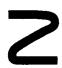
\includegraphics[keepaspectratio]{images/part002_fffac8d3.jpg}}

\begin{enumerate}
\def\labelenumi{\arabic{enumi})}
\setcounter{enumi}{1}
\tightlist
\item
  显然，由半范数 \(N_{\infty}\) 定义的拓扑细于依测度收敛的拓扑在 \(L_{F}^{\infty}\) 上诱导的拓扑（§5, No.~11）。
\end{enumerate}

\subsection{Hölder 不等式}

在本节中，p 与 q 将表示满足 \(1 \leqslant p \leqslant +\infty\)、\(1 \leqslant q \leqslant +\infty\) 且以关系 \(1/p + 1/q = 1\) 相联系的两个实数；于是 \(q = p/(p - 1)\)（若 \(1 < p < +\infty\)），\(q = +\infty\)（若 p = 1），q = 1（若 \(p = +\infty\)）；p 与 q 称为共轭指数。注意，关系 \(1 \leqslant p \leqslant 2\) 等价于 \(2 \leqslant q \leqslant +\infty\)；仅当 p 与 q 都等于 2 时才有 p = q。

定理 2（Hölder 不等式）. --- 设 \(f\) 与 \(g\) 是两个几乎处处有限的数值函数，且 \(f\) 几乎处处等于 \(\mathcal{L}^p\) 中的一个函数，\(g\) 几乎处处等于 \(\mathcal{L}^q\) 中的一个函数。则函数 \(fg\)（几乎处处有定义）可积，且

\[
\mathrm{N} _ {1} (f g) \leqslant \mathrm{N} _ {p} (f) \mathrm{N} _ {q} (g).\tag{4}
\]

设 \(f_{1}\)（相应地，\(g_{1}\)）是 \(\mathcal{L}^{p}\)（相应地，\(\mathcal{L}^{q}\)）中的一个函数，\(f\)（相应地，\(g\)）几乎处处等于它；\(fg\) 几乎处处等于函数 \(f_{1}g_{1}\)，后者处处有定义且有限，且作为两个可测函数的乘积是可测的（§5, No.~3, 定理 1 的推论 5）。若 \(1 < p < +\infty\)，则关于上积分的 Hölder 不等式（Ch. I, No.~3, 命题 4）给出不等式 (4)，而关系式 \(N_{1}(fg) < +\infty\) 这时表明 \(fg\) 可积（§5, No.~6, 定理 5）。若 \(p = 1\)、\(q = +\infty\)，则不等式 (4) 以及 \(fg\) 可积这一事实是平均不等式（No.~2, 命题 1）的直接推论；于是定理在所有情形都得到证明。

推论 1. --- 设 F、G、H 是三个 Banach 空间，\((\mathbf{u}, \mathbf{v}) \mapsto \Phi(\mathbf{u}, \mathbf{v})\) 是 \(F \times G\) 到 H 中的一个连续双线性映射，使得 \(|\Phi(\mathbf{u}, \mathbf{v})| \leqslant |\mathbf{u}| \cdot |\mathbf{v}|\) 。若 \(f \in L_{F}^{p}\) 且 \(g \in L_{G}^{q}\)，则函数 \(\Phi(\mathbf{f}, \mathbf{g})\) 可积，且

\[
\left| \int \Phi (\mathbf {f}, \mathbf {g}) d \mu \right| \leqslant \int | \Phi (\mathbf {f}, \mathbf {g}) | d | \mu | \leqslant \mathrm{N} _ {p} (\mathbf {f}) \mathrm{N} _ {q} (\mathbf {g}).\tag{5}
\]

因为，\(\Phi(\mathbf{f},\mathbf{g})\) 可测（§5, No.~3, 定理 1 的推论 5）；由于 \(|\Phi(\mathbf{f},\mathbf{g})| \leqslant |\mathbf{f}| \cdot |\mathbf{g}|\)，该推论由定理 2 与 §5, No.~6 定理 5 的可积性判别法得出。

推论 1 的两个特殊情形在应用中很重要：

推论 2. --- 设 F 是一个实（相应地，复）Banach 空间，F' 是它的强对偶（TVS, III, §3, No.~1），\((\mathbf{z}, \mathbf{z}') \mapsto \langle \mathbf{z}, \mathbf{z}' \rangle\) 是 \(F \times F'\) 上的规范双线性型。若 \(f \in L_{F}^{p}\) 且 \(g \in L_{F'}^{q}\)，则实（相应地，复）函数 \(\langle f, g \rangle\) 可积，且

\[
\left| \int \langle \mathbf {f}, \mathbf {g} \rangle d \mu \right| \leqslant \int | \langle \mathbf {f}, \mathbf {g} \rangle | d | \mu | \leqslant N _ {p} (\mathbf {f}) N _ {q} (\mathbf {g}).\tag{6}
\]

因为，\(|\langle \mathbf{z},\mathbf{z}^{\prime}\rangle |\leqslant |\mathbf{z}|\cdot |\mathbf{z}^{\prime}|\)

当 F 是一个实或复 Hilbert 空间时，我们知道它可以与它的对偶 \(F'\) 规范地等同（TVS, V, §1, No.~7）。由于空间 \(L_{F}^{2}\) 完备，我们有下列结果：

推论 3. --- 设 \(\mu\) 是 X 上的一个正测度，F 是一个实（相应地，复）Hilbert 空间。在空间 \(L_{F}^{2}\) 上，对称（相应地，Hermite）型

\[
(\widetilde {\mathbf {f}}, \widetilde {\mathbf {g}}) \mapsto \int \langle \mathbf {f}, \mathbf {g} \rangle d \mu
\]

定义了一个 Hilbert 空间结构，其范数等于 \(\| \widetilde{\mathbf{f}}\| _2\)

推论 4. --- 设 F 是一个 Banach 空间，f 是 \(\mathcal{L}_{\mathrm{F}}^{p}\) 中的一个函数，g 是属于 \(\mathcal{L}^q\) 的一个数值函数；则函数 fg 可积，且

\[
\left| \int \mathbf {f} g d \mu \right| \leqslant \int | \mathbf {f} g | d | \mu | \leqslant \mathrm{N} _ {p} (\mathbf {f}) \mathrm{N} _ {q} (g).\tag{7}
\]

推论 5. --- 设 \(f_1, f_2, \ldots, f_n\) 是 \(n\) 个正的可积函数，\(\alpha_1, \alpha_2, \ldots, \alpha_n\) 是 \(n\) 个数 \(> 0\)，使得 \(\sum_{i=1}^{n} \alpha_i = 1\)；在这些条件下，函数 \(f_1^{\alpha_1} f_2^{\alpha_2} \cdots f_n^{\alpha_n}\) 可积，且

\[
\begin{array}{l} \int f _ {1} ^ {\alpha_ {1}} f _ {2} ^ {\alpha_ {2}} \dots f _ {n} ^ {\alpha_ {n}} d | \mu | \leqslant \\ \left(\int f _ {1} d | \mu |\right) ^ {\alpha_ {1}} \left(\int f _ {2} d | \mu |\right) ^ {\alpha_ {2}} \dots \left(\int f _ {n} d | \mu |\right) ^ {\alpha_ {n}}. \end{array}\tag{8}
\]

因为，乘积 \(f_{1}^{\alpha_{1}}f_{2}^{\alpha_{2}}\cdots f_{n}^{\alpha_{n}}\) 作为可测函数的乘积是可测的（§5, No.~3, 定理 1 及其推论 5）；由于不等式 (8) 对上积分成立（Ch. I, No.~2, 命题 2 的推论），函数 \(f_{1}^{\alpha_{1}}f_{2}^{\alpha_{2}}\cdots f_{n}^{\alpha_{n}}\) 可积（§5, No.~6, 定理 5），推论得证。

定理 2 的推论 2 可由下列命题加以强化：

命题 3. --- 设 \(\mu\) 是 X 上的一个正测度，F 是一个实或复 Banach 空间，F' 是它的强对偶，\((\mathbf{z},\mathbf{z}')\mapsto\langle\mathbf{z},\mathbf{z}'\rangle\) 是 F × F' 上的规范双线性型。

\(1^{\circ}\) 对每个函数 \(\mathbf{f} \in \mathcal{L}_{\mathrm{F}}^{p}\)（ \(1 \leqslant p \leqslant +\infty\)），

\[
\mathrm{N} _ {p} (\mathbf {f}) = \sup \left| \int \langle \mathbf {f}, \mathbf {g} \rangle d \mu \right|\tag{9}
\]

其中 \(\mathbf{g}\) 取遍 \(\mathcal{L}_{\mathrm{F}'}^q\) 中满足 \(\mathrm{N}_q(\mathbf{g}) \leqslant 1\) 的函数所成之集。

\(2^{\circ}\) 对每个函数 \(\mathbf{g} \in \mathcal{L}_{\mathrm{F}}^{q}\)（ \(1 \leqslant q \leqslant +\infty\)），

\[
\mathrm{N} _ {q} (\mathbf {g}) = \sup \left| \int \langle \mathbf {f}, \mathbf {g} \rangle d \mu \right|\tag{10}
\]

其中 \(\mathbf{f}\) 取遍 \(\mathcal{L}_{\mathrm{F}}^{p}\) 中满足 \(\mathrm{N}_p(\mathbf{f})\leqslant 1\) 的函数所成之集。

我们先证明关系式 (9)；分两种情形。

\begin{enumerate}
\def\labelenumi{(\roman{enumi})}
\tightlist
\item
  \(1 \leqslant p < +\infty\) 。由于当 \(\mathrm{N}_p(\mathbf{f}) = 0\) 时关系式 (9) 是平凡的（因为这时 \(\mathbf{f}\) 与 \(\langle \mathbf{f}, \mathbf{g} \rangle\) 都可忽略），我们总可以通过用标量乘 \(\mathbf{f}\) 而假设 \(\mathrm{N}_p(\mathbf{f}) = 1\) 。先设 \(\mathbf{f}\) 是一个可积阶梯函数，\(\mathbf{f} = \sum_{k=1}^{n} \dot{\mathbf{a}}_k \varphi_{\mathrm{A}_k}\)，其中诸 \(\mathrm{A}_k\) 两两不相交（§4, No.~9, 引理）。于是按假设 \(\sum_{k=1}^{n} |\mathbf{a}_k|^p \mu(\mathrm{A}_k) = 1\)。对每个 \(\varepsilon > 0\)，（对每个指标 \(k\)）存在向量 \(\mathbf{a}_k' \in \mathrm{F}'\)，使 \(|\mathbf{a}_k'|^q = |\mathbf{a}_k|^p\)（若 \(p > 1\)；相应地，\(|\mathbf{a}_k'| = 1\) 若 \(p = 1\)），且 \(\langle \mathbf{a}_k, \mathbf{a}_k' \rangle \geqslant (1 - \varepsilon) |\mathbf{a}_k| \cdot |\mathbf{a}_k'|\)（TVS, IV, §1, No.~3, 命题 8）。令 \(\mathbf{g} = \sum_{k=1}^{n} \mathbf{a}_{k}^{\prime} \varphi_{\mathrm{A}_{k}}\)，则 \(\sum_{k=1}^{n} |\mathbf{a}_{k}^{\prime}|^{q} \mu(\mathrm{A}_{k}) = 1\)（若 \(p > 1\)；相应地，\(\sup_{1 \leqslant k \leqslant n} |\mathbf{a}_{k}^{\prime}| = 1\) 若 \(p = 1\)），于是 \(\mathrm{N}_{q}(\mathbf{g}) = 1\)；另一方面，
\end{enumerate}

\[
\int \langle \mathbf {f}, \mathbf {g} \rangle d \mu = \sum_ {k = 1} ^ {n} \left\langle \mathbf {a} _ {k}, \mathbf {a} _ {k} ^ {\prime} \right\rangle \mu \left(\mathrm{A} _ {k}\right) \geqslant (1 - \varepsilon) \sum_ {k = 1} ^ {n} | \mathbf {a} _ {k} | \cdot | \mathbf {a} _ {k} ^ {\prime} | \mu (\mathrm{A} _ {k})
\]

又由于 \(|\mathbf{a}_k'| = |\mathbf{a}_k|^{p / q} = |\mathbf{a}_k|^{p - 1}\)（若 \(p > 1\)；相应地，\(|\mathbf{a}_k'| = 1\) 若 \(p = 1\)），我们有

\[
\int \langle \mathbf {f}, \mathbf {g} \rangle d \mu \geqslant (1 - \varepsilon) \sum_ {k = 1} ^ {n} | \mathbf {a} _ {k} | ^ {p} \mu (\mathrm{A} _ {k}) = (1 - \varepsilon) \mathrm{N} _ {p} (\mathbf {f}) = 1 - \varepsilon ,
\]

这就证明了此情形下的关系式 (9)。

再设 \(\mathbf{f}\) 是 \(\mathcal{L}_{\mathrm{F}}^{p}\) 中使 \(\mathrm{N}_p(\mathbf{f}) = 1\) 的任意元素。对每个 \(\varepsilon > 0\)，存在阶梯函数 \(\mathbf{f}_1 \in \mathcal{L}_{\mathrm{F}}^p\)，使 \(\mathrm{N}_p(\mathbf{f} - \mathbf{f}_1) \leqslant \varepsilon\)（§4, No.~10, 命题 19 的推论 1）。由刚才所证，存在函数 \(\mathbf{g} \in \mathcal{L}_{\mathrm{F}}^q\)，使 \(\mathrm{N}_q(\mathbf{g}) = 1\)，且

\[
\int \langle \mathbf {f} _ {1}, \mathbf {g} \rangle d \mu \geqslant \mathrm{N} _ {p} (\mathbf {f} _ {1}) - \varepsilon \geqslant 1 - 2 \varepsilon .
\]

而

\[
\int \left\langle \mathbf {f}, \mathbf {g} \right\rangle d \mu = \int \left\langle \mathbf {f} _ {1}, \mathbf {g} \right\rangle d \mu + \int \left\langle \mathbf {f} - \mathbf {f} _ {1}, \mathbf {g} \right\rangle d \mu
\]

且由 (6)，

\[
\left| \int \langle \mathbf {f} - \mathbf {f} _ {1}, \mathbf {g} \rangle d \mu \right| \leqslant \mathrm{N} _ {p} (\mathbf {f} - \mathbf {f} _ {1}) \mathrm{N} _ {q} (\mathbf {g}),
\]

由此得

\[
\left| \int \langle \mathbf {f}, \mathbf {g} \rangle d \mu \right| \geqslant 1 - 3 \varepsilon ,
\]

这就证明了 (9)。

\begin{enumerate}
\def\labelenumi{(\roman{enumi})}
\setcounter{enumi}{1}
\tightlist
\item
  \(p = +\infty\) 。我们仍可只限于 \(\mathrm{N}_{\infty}(\mathbf{f}) > 0\) 的情形。设 \(\alpha\) 是使 \(0 < \alpha < \mathrm{N}_{\infty}(\mathbf{f})\) 的任一数；按假设，由 \(x \in X\)（满足 \(|\mathbf{f}(x)| > \alpha\) 者）所成之集可测且非局部可忽略，因此它包含一个测度 \textgreater{} 0 的紧集 K。由于 f 可测，存在一个紧集 \(K_{1} \subset K\)（测度 \textgreater{} 0 的），使 f 到 \(K_{1}\) 上的限制连续。由此推出，对每个 \(\varepsilon > 0\)，存在 \(K_{1}\) 分成有限个可积集的一个分割，使 f 在每个集上的振幅 \(\leqslant \varepsilon\)；这些集中至少有一个集 A 的测度 \(>0\)。设 \(\mathbf{a}\) 是 \(\mathbf{f}\) 在 \(\mathbf{A}\) 上的一个值；则 \(|\mathbf{a}| > \alpha\)，且 \(|\mathbf{f}(x) - \mathbf{a}| \leqslant \varepsilon\) 对所有 \(x \in \mathbf{A}\) 成立。存在向量 \(\mathbf{a}' \in \mathbf{F}'\)，使 \(|\mathbf{a}'| = 1\) 且 \(|\langle \mathbf{a}, \mathbf{a}' \rangle| \geqslant |\mathbf{a}| - \varepsilon\)；函数 \(\mathbf{g} = \varphi_{\mathrm{A}} \cdot \mathbf{a}' / \mu(\mathbf{A})\) 可积且 \(\mathrm{N}_1(\mathbf{g}) = 1\)；另一方面，
\end{enumerate}

\[
\int \langle \mathbf {f}, \mathbf {g} \rangle d \mu = \frac {1}{\mu (\mathrm{A})} \int \langle \mathbf {f}, \mathbf {a} ^ {\prime} \rangle \varphi_ {\mathrm{A}} d \mu .
\]

而我们可以写出

\[
\int \langle {\bf f}, {\bf a} ^ {\prime} \rangle \varphi_ {\mathrm{A}} d \mu = \langle {\bf a}, {\bf a} ^ {\prime} \rangle \mu (\mathrm{A}) + \int \langle {\bf f} - {\bf a}, {\bf a} ^ {\prime} \rangle \varphi_ {\mathrm{A}} d \mu ,
\]

且由于

\[
\left| \langle \mathbf {f} - \mathbf {a}, \mathbf {a} ^ {\prime} \rangle \varphi_ {\mathrm{A}} \right| \leqslant \varepsilon \varphi_ {\mathrm{A}},
\]

我们看出

\[
\left| \int \langle \mathbf {f}, \mathbf {g} \rangle d \mu \right| \geqslant | \langle \mathbf {a}, \mathbf {a} ^ {\prime} \rangle | - \varepsilon \geqslant | \mathbf {a} | - 2 \varepsilon > \alpha - 2 \varepsilon ;
\]

由于 \(\varepsilon\) 任意而 \(\alpha\) 是任何 \(<\mathrm{N}_{\infty}(\mathbf{f})\) 的数，关系式 (9) 在此情形也得到验证。

证明关系式 (10) 的方式完全相同：分别考虑 \(1 \leqslant q < +\infty\) 与 \(q = +\infty\) 两种情形，并利用如下事实：对每个 \(\mathbf{z}' \in \mathrm{F}'\)，有 \(|\mathbf{z}'| = \sup_{|\mathbf{z}| \leqslant 1} |\langle \mathbf{z}, \mathbf{z}' \rangle|\)（由 \(\mathrm{F}'\) 中范数的定义）。

注. --- 1) 设 \(\mathcal{E}\) 是 \(\mathcal{L}_{\mathrm{F}'}^q\) 的一个稠密线性子空间；则当 \(\mathbf{g}\) 取遍 \(\mathcal{E}\) 与集 B——\(\mathcal{L}_{\mathrm{F}'}^q\) 中满足 \(\mathrm{N}_q(\mathbf{g}) \leqslant 1\) 的函数所成者——的交时，公式 (9) 成立。因为，只需注意到 B 的内部 \(\overset{\circ}{\mathrm{B}}\) 在 B 中稠密，且 \(\overset{\circ}{\mathrm{B}} \cap \mathcal{E}\) 在 \(\overset{\circ}{\mathrm{B}}\) 中稠密（因为 \(\overset{\circ}{\mathrm{B}}\) 是开的）。这一注记特别适用于集 \(\mathcal{E} = \mathcal{K}(\mathrm{X};\mathrm{F}')\)——由具紧支集的连续函数（取值于 \(\mathrm{F}'\)）所成者——（当 \(1 \leqslant q < +\infty\)，即 \(1 < p \leqslant +\infty\) 时）。但在这一情形，公式 (9) 当 \(\mathbf{g}\) 取遍 \(\mathrm{B} \cap \mathcal{K}(\mathrm{X};\mathrm{F}')\) 时成立，甚至对 \(p = 1\) 也如此。因为，我们可以如同上面那样只限于 \(\mathbf{f}\) 是阶梯函数的情形。这时我们看到，若 \(\mathrm{N}_1(\mathbf{f}) = 1\)，则对每个 \(\varepsilon > 0\)，存在阶梯函数 \(\mathbf{g} \in \mathcal{L}_{\mathrm{F}'}^{\infty}\)，使得 \(|\mathbf{g}(x)| \leqslant 1\) 对所有 \(x \in \mathrm{X}\) 成立，且 \(|\int \langle \mathbf{f},\mathbf{g}\rangle d\mu| \geqslant 1 - \varepsilon\) 。存在有限个两两不相交的紧集 \(\mathrm{K}_i\)，使 \(\mathbf{g}\) 取常值 \(\mathbf{a}_i'\)（在每个 \(\mathrm{K}_i\) 上），且若 K 是诸 \(\mathrm{K}_i\) 之并，则 \(\int |\mathbf{f}| \varphi_{\mathbf{C} K} d\mu \leqslant \varepsilon\) 。设 \(\mathrm{U}_i\) 是 \(\mathrm{K}_i\) 的一个邻域，使诸 \(\mathrm{U}_i\) 两两不相交，并设 \(h_i\) 是 X 到 {[}0,1{]} 中的一个连续映射，其支包含于 \(\mathrm{U}_i\) 且在 \(\mathrm{K}_i\) 上等于 1。令 \(\mathbf{h} = \sum \mathbf{a}_i' h_i\)，则在 K 上 \(\mathbf{h}(x) = \mathbf{g}(x)\)，且在 X 上 \(|\mathbf{h}(x)| \leqslant 1\)，因此

\[
\int | \langle \mathbf {f}, \mathbf {h} \rangle | \varphi_ {\mathbf {C K}} d \mu \leqslant \varepsilon
\]

从而 \(|\int \langle \mathbf{f},\mathbf{h}\rangle d\mu |\geqslant 1 - 3\varepsilon\)，这就证明了我们的断言。对公式 (10) 可作类似的注记。

\begin{enumerate}
\def\labelenumi{\arabic{enumi})}
\setcounter{enumi}{1}
\tightlist
\item
  设 \(\mu\) 是 \(X\) 上的一个正测度，\(f\) 是一个可测函数 \(\geqslant 0\)（有限或无限），其支集含于紧集 \(K_{n}\) 的一个可数并。则对每个 \(p\)（满足 \(1 \leqslant p \leqslant +\infty\) 者），
\end{enumerate}

\[
\mathrm{N} _ {p} (f) = \sup \int^ {*} | f g | d \mu ,\tag{11}
\]

其中 \(g\) 取遍 \(\mathcal{K}(\mathrm{X};\mathbf{R})\) 中满足 \(\mathrm{N}_q(g)\leqslant 1\) 的函数所成之集。因为，当 \(\mathrm{N}_p(f) < +\infty\) 时公式 (11) 是 (9) 的特殊情形，因为这时 \(f\) 等价于 \(\mathcal{L}^p\) 中的一个函数（§5, No.~6, 定理 5）。若 \(\mathrm{N}_p(f) = +\infty\)，对每个整数 \(n > 0\) 令 \(f_{n} = \inf (n,f\varphi_{\mathrm{K}_{n}})\) 。则

\[
\mathrm{N} _ {p} (f _ {n}) = \sup \int^ {*} | f _ {n} g | d \mu \leqslant \sup \int^ {*} | f g | d \mu ,
\]

于是（假设如我们所可以的那样，序列 \((\mathbf{K}_n)\) 递增）过渡到极限，便得 \(\sup \int^{*}|fg| d\mu = +\infty\)（§1, No.~3, 定理 3）。

推论. --- 设 \(\mu\) 是 X 上的一个正测度，F 是一个 Banach 空间，\(F'\) 是它的强对偶，g 是 \(L_{F'}^{q}\) 中的任一函数。则由 \(L_{F}^{p}\) 上的线性形式 \(f \mapsto \int \langle f, g \rangle d\mu\) 过渡到商得到的 \(L_{F}^{p}\) 上的线性形式是连续的，且范数为 \(N_{q}(g)\) 。

\subsection{\texorpdfstring{应用：空间 \(\mathcal{L}_{F}^{p}\) （ \(1 \leqslant p \leqslant +\infty\) ）之间的关系}{应用：空间 L sub F to the p （ 1 <= p <= +infinity ）之间的关系}}

命题 4. --- 设 f 是以一个 Banach 空间 F 为值的可测函数；使 \(1 \leqslant p \leqslant +\infty\) 且 \(\mathrm{N}_{p}(\mathbf{f})\) 有限的数 p 所成之集 I，或为空，或为 \(\overline{R}\) 的一个区间。若 I 非空，则映射 \(p \mapsto \mathrm{N}_{p}(\mathbf{f})\) 在 I 上的限制连续；此外，若 f 非可忽略，则 \(\log \mathrm{N}_{p}(\mathbf{f})\) 是 1/p 在 \(\overline{I}\) 上的凸函数。

我们已经知道（Ch. I, No.~3, 命题 5），有限数 \(p \geqslant 1\)（使 \(\mathrm{N}_{p}(\mathbf{f}) < +\infty\) 者）所成之集 J 或为空，或为一个区间，且 \(\log \mathrm{N}_{p}(\mathbf{f})\) 是 1/p 在 J 上的凸函数（当 f 非可忽略时）；这当然蕴涵 \(p \mapsto \mathrm{N}_{p}(\mathbf{f})\) 在 J 上的连续性。

若 J 为空，则或者 \(I = \varnothing\)，或者 \(I = \{+\infty\}\)，命题在此情形是显然的；以下设 J 非空。若 f 可忽略，命题也是显然的；以下设 f 非可忽略。若 \(s \in J\)，则对每个有限数 p \textgreater{} s，\(|f|^{p} = |f|^{s}|f|^{p-s}\)，且平均不等式表明

\[
\mathrm{N} _ {p} (\mathbf {f}) \leqslant \left(\mathrm{N} _ {s} (\mathbf {f})\right) ^ {s / p} \left(\mathrm{N} _ {\infty} (\mathbf {f})\right) ^ {(p - s) / p}.\tag{12}
\]

令 \(p\) 趋于 \(+\infty\)，由此得出

\[
\limsup _ {p \to + \infty} N _ {p} (\mathbf {f}) \leqslant N _ {\infty} (\mathbf {f})  .\tag{13}
\]

这就证明了：若 \(+\infty \in I\)，则 \(J\) 含有任意大的数；于是 \(I\) 确是 \(\overline{\mathbf{R}}\) 的一个区间，且 \(\overline{I} = \overline{J}\) 。若我们能证明 \(p \mapsto N sub p(\mathbf{f})\) 在 \(\overline{J}\) 上连续，命题即告证明；而只需在 \(J\) 的端点处建立连续性。此外，我们还可以假设 \(J\) 不退缩为一点。设 \(r\) 与 \(s\) 是 \(J\) 的左、右端点（ \(r < s \leqslant +\infty\)）。设 \(A\) 是由 \(x \in X\)（满足 \(|\mathbf{f}(x)| \geqslant 1\) 者）所成之（可测）集；则

\[
\int | \mathbf {f} | ^ {p} d | \mu | = \int | \mathbf {f} | ^ {p} \varphi_ {\mathrm{A}} d | \mu | + \int | \mathbf {f} | ^ {p} \varphi_ {\mathbf {C A}} d | \mu |.
\]

当 \(p \in \mathbf{J}\) 趋于 \(r\) 时，\(|\mathbf{f}|^p\varphi_{\mathbf{A}}\) 递减地趋于 \(|\mathbf{f}|^r\varphi_{\mathbf{A}}\)，而 \(|\mathbf{f}|^p\varphi_{\mathbf{C}_{\mathbf{A}}}\) 递增地趋于 \(|\mathbf{f}|^r\varphi_{\mathbf{C}_{\mathbf{A}}}\)。于是 \(\int |\mathbf{f}|^p\varphi_{\mathbf{C}_{\mathbf{A}}}d|\mu|\) 趋于 \(\int^{*}|\mathbf{f}|^{r}\varphi_{\mathbf{C}_{\mathbf{A}}}d|\mu|\)（§1, No.~3, 定理 3）。另一方面，\(|\mathbf{f}|^p\varphi_{\mathbf{A}}\) 对 \(p \in \mathbf{J}\) 可积，且 \(\int |\mathbf{f}|^p\varphi_{\mathbf{A}}d|\mu|\) 趋于 \(\int |\mathbf{f}|^r\varphi_{\mathbf{A}}d|\mu|\)（§4, No.~3, 命题 4）。因此 \(\int |\mathbf{f}|^p d|\mu|\) 趋于 \(\int^{*}|\mathbf{f}|^{r}d|\mu|\)，这就证明了 \(p \mapsto \mathrm{N}_p(\mathbf{f})\) 在 \(r\) 处的连续性。

同样的推理可应用于点 \(s\)（若 \(s < +\infty\)）。最后，设 \(s = +\infty\) 。鉴于 (13)，只需证明

\[
\liminf _ {p \to + \infty} N _ {p} (\mathbf {f}) \geqslant N _ {\infty} (\mathbf {f}).
\]

而设 \(a\) 是使 \(0 < a < \mathrm{N}_{\infty}(\mathbf{f})\) 的一个数。由于按假设存在有限值 \(p\)（使 \(\mathrm{N}_p(\mathbf{f}) < +\infty\) 者），故集 \(A\)——由 \(x \in X\)（满足 \(|\mathbf{f}(x)| \geqslant a\) 者）组成，它可测且非可忽略——由不等式 \(\varphi_A \leqslant (|\mathbf{f}|/a)^p\) 是可积的；此外，由这一不等式推出 \(\mathrm{N}_p(\mathbf{f}) \geqslant a \cdot (|\mu|(\mathrm{A}))^{1/p}\)；令 \(p\) 趋于 \(+\infty\)，得 \(\liminf_{p \to +\infty} \mathrm{N}_p(\mathbf{f}) \geqslant a\)，证毕。

推论. --- 若 r, s, p 是满足

\[
1 \leqslant r <   p <   s \leqslant + \infty ,
\]

的三个数，则交 \(\mathcal{L}_{\mathrm{F}}^{r} \cap \mathcal{L}_{\mathrm{F}}^{s}\) 含于 \(\mathcal{L}_{\mathrm{F}}^{p}\) 。

注意，一般说来，在交 \(\mathcal{L}_{\mathrm{F}}^{r} \cap \mathcal{L}_{\mathrm{F}}^{s}\) 上由诸 \(\mathcal{L}_{\mathrm{F}}^{p}\)（ \(r < p < s\)）的拓扑诱导的拓扑互不相同。若对 \(\mu\) 不再作任何假设，则在 \(\mathcal{L}_{\mathrm{F}}^{r} \cap \mathcal{L}_{\mathrm{F}}^{s}\) 上由 \(\mathcal{L}_{\mathrm{F}}^{r}\) 与 \(\mathcal{L}_{\mathrm{F}}^{s}\) 的拓扑诱导的拓扑一般不可比较（换句话说，商 \(\mathrm{N}_{r}(\mathbf{f})/\mathrm{N}_{s}(\mathbf{f})\) 在 \(L_{F}^{r} \cap L_{F}^{s}\) 中可取到任意大的值与任意小的值；参见习题 8）。

当 \(\mu\) 是有界测度时，命题 4 可以加强：

命题 5. --- 设 \(\mu\) 是一个有界测度，\(\mathbf{f}\) 是一个 \(\mu\)-可测函数（以 Banach 空间 \(\mathbf{F}\) 为值的）。数 \(p\)（满足 \(1 \leqslant p \leqslant +\infty\) 且 \(\mathrm{N}_p(\mathbf{f})\) 有限者）所成之集 I，或为空，或为以 \(p = 1\) 为左端点且含该点的区间；此外，\((|\mu|(\mathrm{X}))^{-1/p} \mathrm{N}_p(\mathbf{f})\) 是 \(p\) 在 I 上的递增函数。

这是上面命题 4 与 Ch. I, No.~3 命题 4 的推论的直接推论。

推论. --- 若测度 \(\mu\) 有界，则关系 r < s 蕴涵 \(L_{F}^{s} \subset L_{F}^{r}\)；此外，s 阶平均收敛的拓扑细于 r 阶平均收敛的拓扑（在 \(L_{F}^{s}\) 上）。

可以证明，一般说来 \(s\) 阶平均收敛的拓扑严格细于 \(r\) 阶平均收敛的拓扑（习题 8）。

命题 6. --- 设 X 是一个离散空间，\(\mu\) 是通过在 X 的每一点放置一个质量 \(+1\) 而定义的 X 上的测度。若 \(\mathbf{f}\) 是 X 到 Banach 空间 F 中的一个映射，则数 \(p\)（满足 \(1 \leqslant p \leqslant +\infty\) 且 \(\mathrm{N}_p(\mathbf{f})\) 有限者）所成之集 I，或为空，或为以 \(+\infty\) 为右端点且含该点的区间；此外，\(\mathrm{N}_p(\mathbf{f})\) 是 \(p\) 在 I 上的递减函数。

因为，\(\mu^{*}(|\mathbf{f}|) = \sum_{x\in X}|\mathbf{f}(x)|\) 对每个函数 \(\mathbf{f}\) 成立（ \(\S 1\) , No.~1, 例），且 \(\mathrm{N}_{\infty}(\mathbf{f}) = \| \mathbf{f}\| = \sup_{x\in X}|\mathbf{f}(x)|\)；若存在数 \(\alpha >0\) 使 \(|\mathbf{f}(x)|\geqslant \alpha\) 对无穷多个 \(x\in X\) 成立，则 \(\mathrm{N}_p(\mathbf{f}) = +\infty\) 对每个有限 \(p\) 成立；在相反的情形，存在 \(x_0\in X\) 使 \(|\mathbf{f}(x_0)| = \| \mathbf{f}\|\)，于是

\[
\mathrm{N} _ {\infty} (\mathbf {f}) = | \mathbf {f} (x _ {0}) | \leqslant \mathrm{N} _ {p} (\mathbf {f})
\]

对每个有限 p 成立。~由于函数 \(\log\mathrm{N}_{p}(\mathbf{f})\) 关于 1/p 是凸的且在点 \(+\infty\) 处取其最小值，它必然是 p 在 I 上的递减函数（FRV, I, §4, No.~3, 命题 5），证毕。

推论. --- 若 X 离散且测度 \(\mu\) 由在 X 的每一点放置质量 +1 而定义，则关系 r < s 蕴涵 \(L_{F}^{r} \subset L_{F}^{s}\)；此外，r 阶平均收敛的拓扑细于 s 阶平均收敛的拓扑（在 \(L_{F}^{r}\) 上）。

\section{重心}

\subsection{重心的定义}

设 E 是 R 上的一个 Hausdorff 局部凸空间，\(E'\) 是它的对偶，\(E'^{*}\) 是 \(E'\) 的代数对偶，E 被规范地等同于 \(E'^{*}\) 的一个线性子空间。设 K 是 E 的一个紧子集；K 到 E 中的规范单射连续且具有紧支集，故对 K 上的每个测度 \(\mu\)，积分 \(\int x d\mu(x)\) 有定义且是 \(E'^{*}\) 的一个元素（Ch. III, §3, No.~1）。此外，在 K 上，由弱拓扑 \(\sigma(E'^{*}, E')\) 诱导的拓扑与原来的拓扑一致。最后，若 C 是 K 在 \(E'^{*}\)（赋以 \(\sigma(E'^{*}, E')\)）中的闭凸包，则 \(C \cap E\) 是 K 在 E 中关于原来的拓扑（或关于弱化拓扑 \(\sigma(E, E')\)）的闭凸包。

定义 1. --- 设 K 是 Hausdorff 局部凸空间 E 的一个紧子集。对 K 上每个总质量等于 1 的正测度 \(\mu\)，向量 \(\mathbf{b}_{\mu} = \int \mathbf{x} d\mu(\mathbf{x})\)（属于 \(E'^{*}\)）称为 \(\mu\) 的重心。

例. --- 设 \(\mu\) 是 K 上的一个离散测度，为正且总质量为 1；于是它形如 \(\mu = \sum_{i=1}^{n} \lambda_i \varepsilon_{x_i}\)，其中 \(x_i \in K\)，诸 \(\lambda_i\) 是实数，满足对一切 i 有 \(\lambda_i \geqslant 0\) 且 \(\sum_{i=1}^{n} \lambda_i = 1\) 。由于 \(\int x d\varepsilon_y(x) = y\)（Ch. III, §3, No.~1, 例 3），\(b_\mu = \int x d\mu(x) = \sum_{i} \lambda_i x_i\) 。特别地，对每个 \(x \in K\)，x 是测度 \(\varepsilon_x\) 的重心。

命题 1. --- 设 E 是一个 Hausdorff 局部凸空间，K 是 E 的一个紧子集，C 是 K 在 E 中的闭凸包。则 C 由 E 中至少是 K 上一个质量为 1 的正测度的重心的那些点组成。

这不过是 Ch. III, §3, No.~2 命题 5 应用于 K 到 E 中的规范单射而已。

推论. --- 若 K 在 E 中的闭凸包 C 是紧的，则 K 上每个总质量为 1 的正测度的重心属于 E。

因为，这时 C 也是 K 在赋以弱拓扑 \(\sigma (\mathrm{E}^{\prime *},\mathrm{E}^{\prime})\) 的 E'* 中的闭凸包，故只需对 K 到 E 中的规范单射应用 Ch. III, §3, No.~2 命题 4。

注. --- 命题 1 的推论特别适用于 K 为凸集或 E 为拟完备的情形。

命题 2. --- 设 K 是 Hausdorff 局部凸空间 E 的一个紧凸子集，\(\mu\) 是 K 上总质量为 1 的一个正测度，\(b_{\mu}\) 是它的重心。对每个在 K 上下半连续的凸数值函数 \(f \geqslant 0\)，

\[
f (\mathbf {b} _ {\mu}) \leqslant \int^ {*} f d \mu .
\]

已知（TVS, II, §5, No.~4, 命题 5）\(f\) 是到 \(K\) 上的限制——连续仿射线性函数 \(h_{\alpha} : \mathbf{x} \mapsto c_{\alpha} + \langle \mathbf{x}, \mathbf{z}_{\alpha}' \rangle\) 的限制——所成族的上包络。则

\[
\int h _ {\alpha} (\mathbf {x}) d \mu (\mathbf {x}) \leqslant \int^ {*} f (\mathbf {x}) d \mu (\mathbf {x})
\]

对每个 \(\alpha\) 成立；而 \(\int h_{\alpha}(\mathbf{x}) d\mu (\mathbf{x}) = c_{\alpha} + \int \langle \mathbf{x}, \mathbf{z}_{\alpha}' \rangle d\mu (\mathbf{x})\)（因为 \(\mu\) 的总质量为 1）；但由重心的定义，\(\int \langle \mathbf{x}, \mathbf{z}_{\alpha}' \rangle d\mu (\mathbf{x}) = \langle \mathbf{b}_{\mu}, \mathbf{z}_{\alpha}' \rangle\)。因此 \(\sup \int h_{\alpha}(\mathbf{x}) d\mu (\mathbf{x}) = \sup h_{\alpha}(\mathbf{b}_{\mu}) = f(\mathbf{b}_{\mu})\)，结论得证。

当 \(\mu\) 是 K 上总质量为 1 的一个离散正测度时，命题 2 重新给出定义 K 上凸函数的那个不等式。

推论. --- 对每个凸数值函数 \(g\)（\(K\) 上的，有界且下半连续），有 \(g(\mathbf{b}_{\mu}) \leqslant \int g d\mu\) 。

只需注意到 \(\inf_{\mathbf{x} \in \mathrm{K}} g(\mathbf{x}) = a\) 有限，并对 \(g - a\) 应用命题 2。
